\documentclass{article}
\usepackage[utf8]{inputenc}
\usepackage{lmodern}
\usepackage[T1]{fontenc}
\usepackage[utf8]{inputenc}
\usepackage[spanish,activeacute]{babel}
\usepackage{titlesec}
\usepackage[obeyspaces]{url}
\usepackage[a4paper, margin=1in]{geometry}
\titleformat{\section}
  {\normalfont\fontsize{14}{14}\bfseries}{\thesection}{1em}{}
\titlespacing{\paragraph}{0pt}{1.5em}{.5em}[]
\titleformat{\paragraph}
{\normalfont\normalsize\bfseries}{\theparagraph}{1em}{}
\titlespacing*{\paragraph}
{0pt}{3.25ex plus 1ex minus .2ex}{1.5ex plus .2ex}
\inputencoding{utf8}
\usepackage{mathtools}
\usepackage{graphicx}
\DeclareGraphicsExtensions{.png,.pdf,.jpg,.webp}
\usepackage{float}
\usepackage{amssymb}
\usepackage{cancel}
\usepackage{bm}
\usepackage{amsmath}
\usepackage{color}
\usepackage{caption}
\usepackage{subcaption}
\usepackage[colorlinks=true,linkcolor=blue]{hyperref}%
\usepackage[toc,title,page]{appendix}
\addto\captionsspanish{%
  \renewcommand\appendixname{Anexo}
  \renewcommand\appendixpagename{Anexos}
  \renewcommand\appendixtocname{Anexos}
}
\usepackage{listingsutf8}
\usepackage{listings}
\renewcommand{\lstlistingname}{Código}
\renewcommand\lstlistlistingname{Códigos fuente}
\definecolor{dkgreen}{rgb}{0,0.6,0}
\definecolor{ltgray}{rgb}{0.5,0.5,0.5}
\hypersetup{
    colorlinks,
    citecolor=black,
    filecolor=black,
    urlcolor=black
}


\title{Taller de Coches}
\author{Martin Fagoaga y Gonzalo Álvarez}
\date{2022}
\begin{document}
\maketitle 
\begin{figure}[H]
  \centering
  \includegraphics[width=1.0\textwidth]{pexels-cottonbro-4480505.jpg}
\end{figure}
\clearpage

{
  \hypersetup{ linkcolor=black}
  \tableofcontents
\clearpage
\listoffigures
\clearpage


}

\section{FASE 1: ANALISIS Y DISEÑO}
\subsection{Introducción: AppTaller}
\subsection{Objetivos}
En este proyecto tenemos como objetivo desarrollar un programa y desplegar una página web para un taller mecánico.
Para ello utilizaremos los contenidos vistos en todas las asignaturas y los conectaremos entre si.\\
El programa debe ser de utilidad para la realización del trabajo del taller, y debería ayudar a mantener un flujo de 
trabajo adecuado.
\subsection{Contextualización del proyecto}
\label{subsection:context}
A la hora de desarrollar una aplicación para un taller mecánico, esta puede englobar todos los ámbitos que conllevan
un taller o centrarse en algún área especifica. En nuestro caso, nos centraremos en lo que es puramente trabajo de taller,
es decir, no pretendemos que nuestra aplicación tenga un uso contable, sino más bien que se trate de una aplicación de 
gestión de reparaciones de vehículos.\\
Por otra parte, la web será puramente informativa y de contacto. Es decir, en ella podrá conocer sobre el taller y los productos que se usan
en el taller, pero no se venderá ningún producto o servicio en la web.
\subsection{Análisis}
El taller que hemos planteado tiene 3 puestos de reparación de vehículos. Por lo tanto, pueden trabajar en 3 vehículos simultaneamente.
Además de ello, tiene una pequeña oficina, donde tienen material típico de oficina como un impresora y donde entra la línea telefónica y de internet.
\begin{figure}[H]
  \centering
  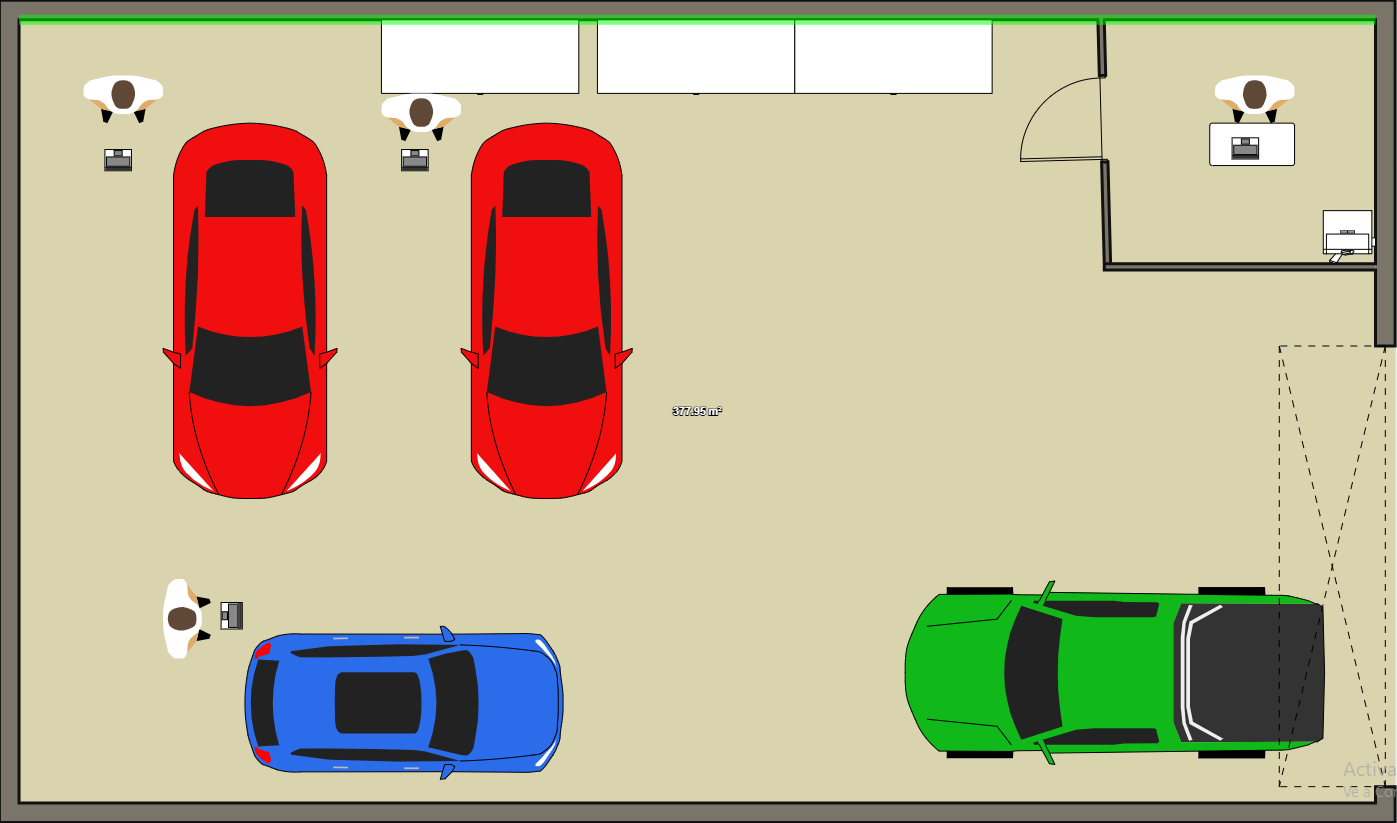
\includegraphics[width=1.0\textwidth]{misc/planoTaller.PNG}
  \caption{Plano del taller.}
\end{figure}
Ya que un taller tiene muchas piezas y herramientas móviles, y se van moviendo de un lado a otro mientras se trabaja, 
hemos decidido que como material para la empresa serán necesarios unos portátiles para los puestos de reparación.\\
La conexión a internet se realizará via Wi-Fi, evitando el cableado y reduciendo el riesgo que tengan los empleados de 
tropezarse, ya que consideramos esta tecnología suficientemente fiable.\\ 
También hemos decidido que contrataremos el alojamiento del servidor a una empresa externa, reduciendo el riesgo de perdida de datos por apagones de 
luz, y reduciendo así el consumo de luz del taller. \\ En cuanto al hardware y software de este material, el servidor deberá correr un sistema linux, 
y los portátiles cualquier sistema operativo en el que instalemos java.
\subsection{Diseño} 
\subsubsection{Diagramas}
En la situación que hemos planteado en la sección \ref{subsection:context}, nos surgen los siguientes casos de uso de una aplicación para los empleados:
\begin{figure}[H]
  \centering
  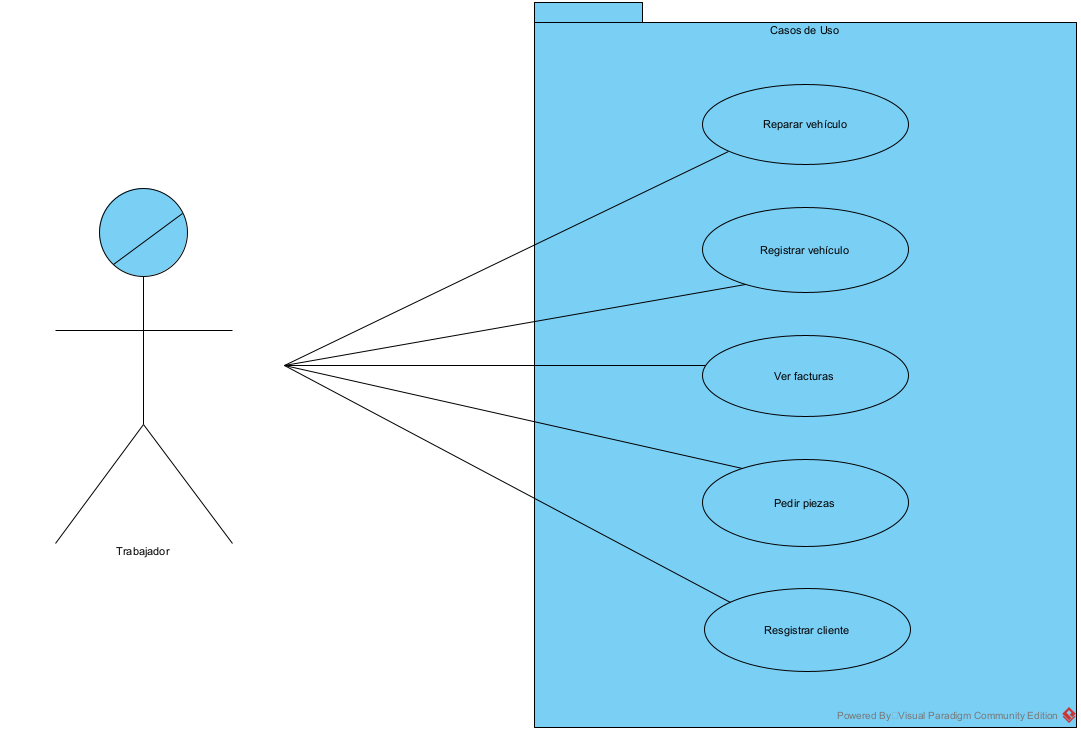
\includegraphics[width=1.0\textwidth]{misc/CasosDeUsoTalleresGutierrez.png}
  \caption{Casos de uso de una aplicación de taller.}
\end{figure}
Debido a que a nosotros se nos demanda implementar un caso de uso, nos centraremos en desarrollar el caso de uso \textbf{reparar vehículo.}.
En el apartado \ref{subsubsection:designClass} especificamos la estructura con la que desarrollaremos el programa e incluimos un diagrama de secuencia para este caso de uso. 
\subsubsection{Modelo DDBB}
Tras analizar el contexto del proyecto, nos hemos decantado por el siguiente modelo E/R: 
\begin{figure}[H]
  \centering
  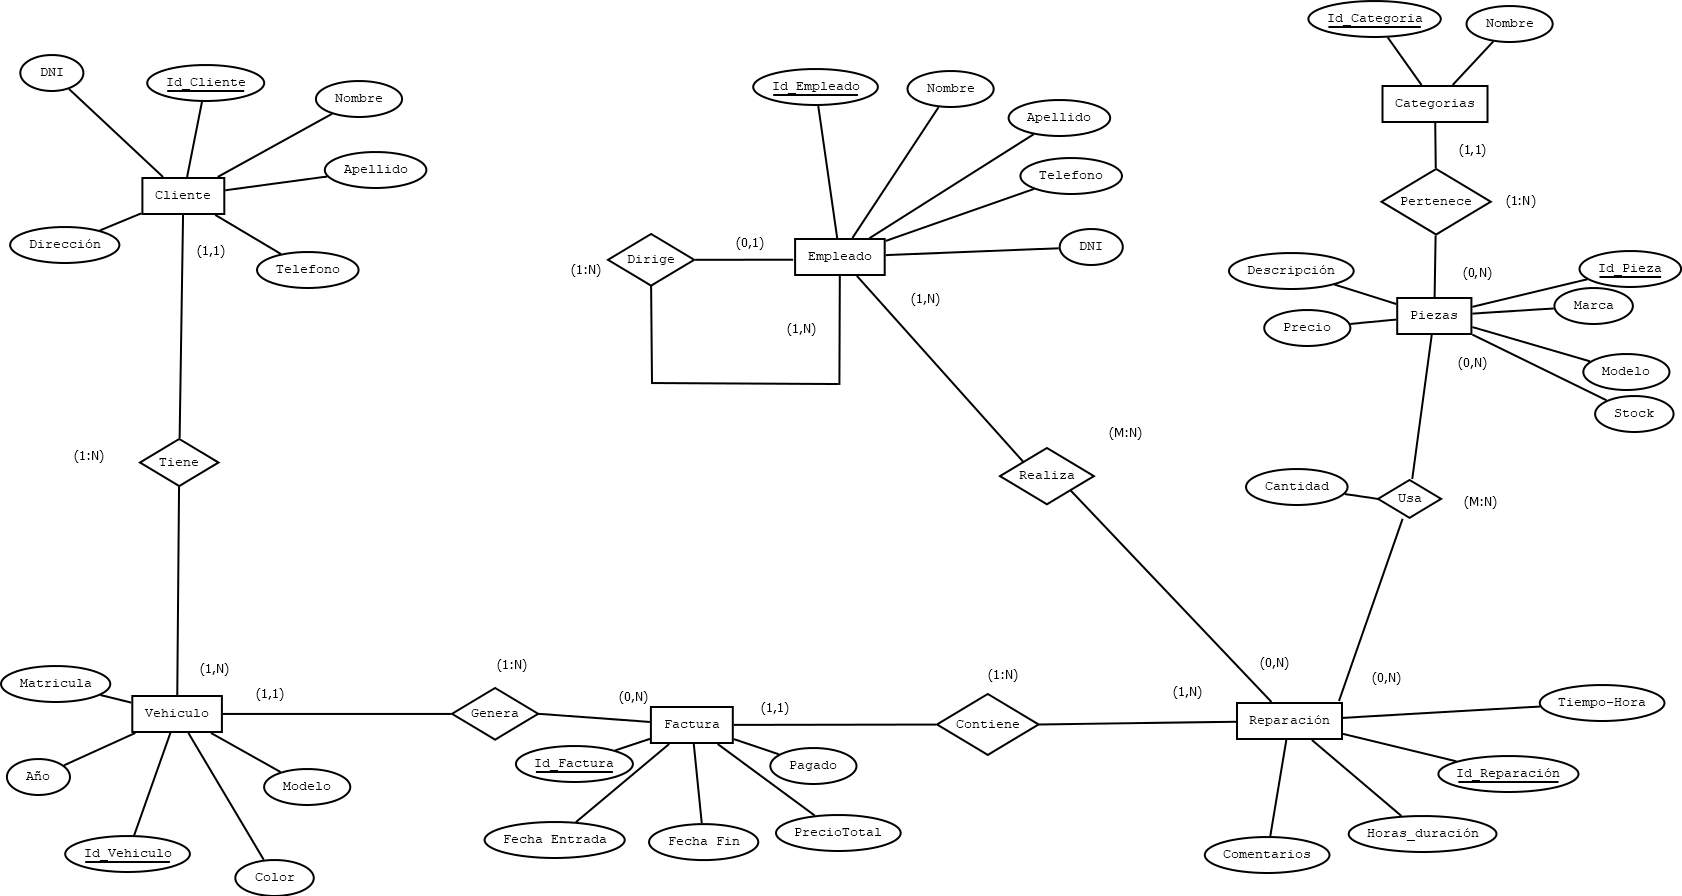
\includegraphics[width=1.0\textwidth]{bbdd/DiagramaEntidadRelacion.png}
  \caption{Diagrama E/R de la BD}
  \label{fig:ER}
\end{figure}
A la hora de decantarnos por este modelo, hemos desechado las siguientes opciones:\\
\begin{itemize}
  \item Proveedores: Hemos decidido no incluir la parte logística de la obtención de piezas. La inclusión complicaría en exceso la base de datos, y teniendo en cuenta que solo debemos implementar un caso de uso, no lo hemos visto necesario.
  \item Salarios: Ya que no hemos incluído lo anterior, hemos decidido no incluir nada relacionado con los gastos de empresa. Hemos decidido que de añadirse, deberiamos añadir todos los gastos para tener una gestión de contabilidad completa.
\end{itemize}
Debido a estas decisiones, hemos decidido enfocar más nuestro proyecto a la parte puramente mecánica y relacionada con el taller de la empresa. Hemos realizado las transformaciones necesarias al diseño E/R, por lo que las 
tablas que tendremos que crear son las siguientes:
\begin{figure}[H]
  \centering
  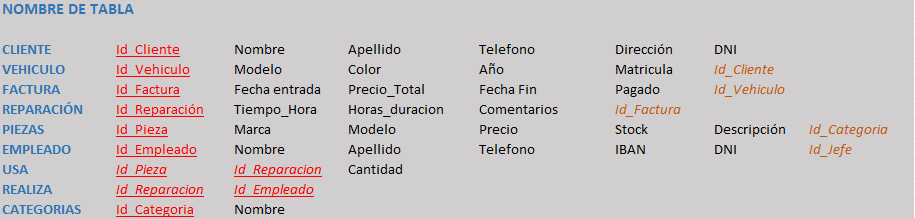
\includegraphics[width=1.0\textwidth]{bbdd/normalizacion.PNG}
  \caption{Normalización del modelo E/R}
\end{figure}
\subsubsection{Diseño de interfaces}
\subsubsection{Listado y Descripción de funcionalidades}
Ya que hemos sido limitados a implementar un caso de uso, al implementar el caso de uso de reparar un vehículo nuestro programa tendrá las siguientes funcionalidades:\\
\begin{itemize}
  \item Elegir un vehículo de la lista de vehículos registrados.
  \item Ver que vehículos están siendo reparados.
  \item Realizar una reparacion: \begin{itemize}
    \item Añadir piezas a la reparación.
    \item Especificar la duración de la reparación.
    \item Añadir comentarios para que el cliente los lea.
  \end{itemize}
  \item Generar una factura en formato .pdf.
\end{itemize}
\subsubsection{Diseño de clases y métodos}
\label{subsubsection:designClass}
Como hemos mencionado anteriormente, solo hemos implementado un caso de uso en nuestro programa. Para ello, hemos diseñado y programado las siguientes clases: 
\begin{figure}[H]
  \centering
  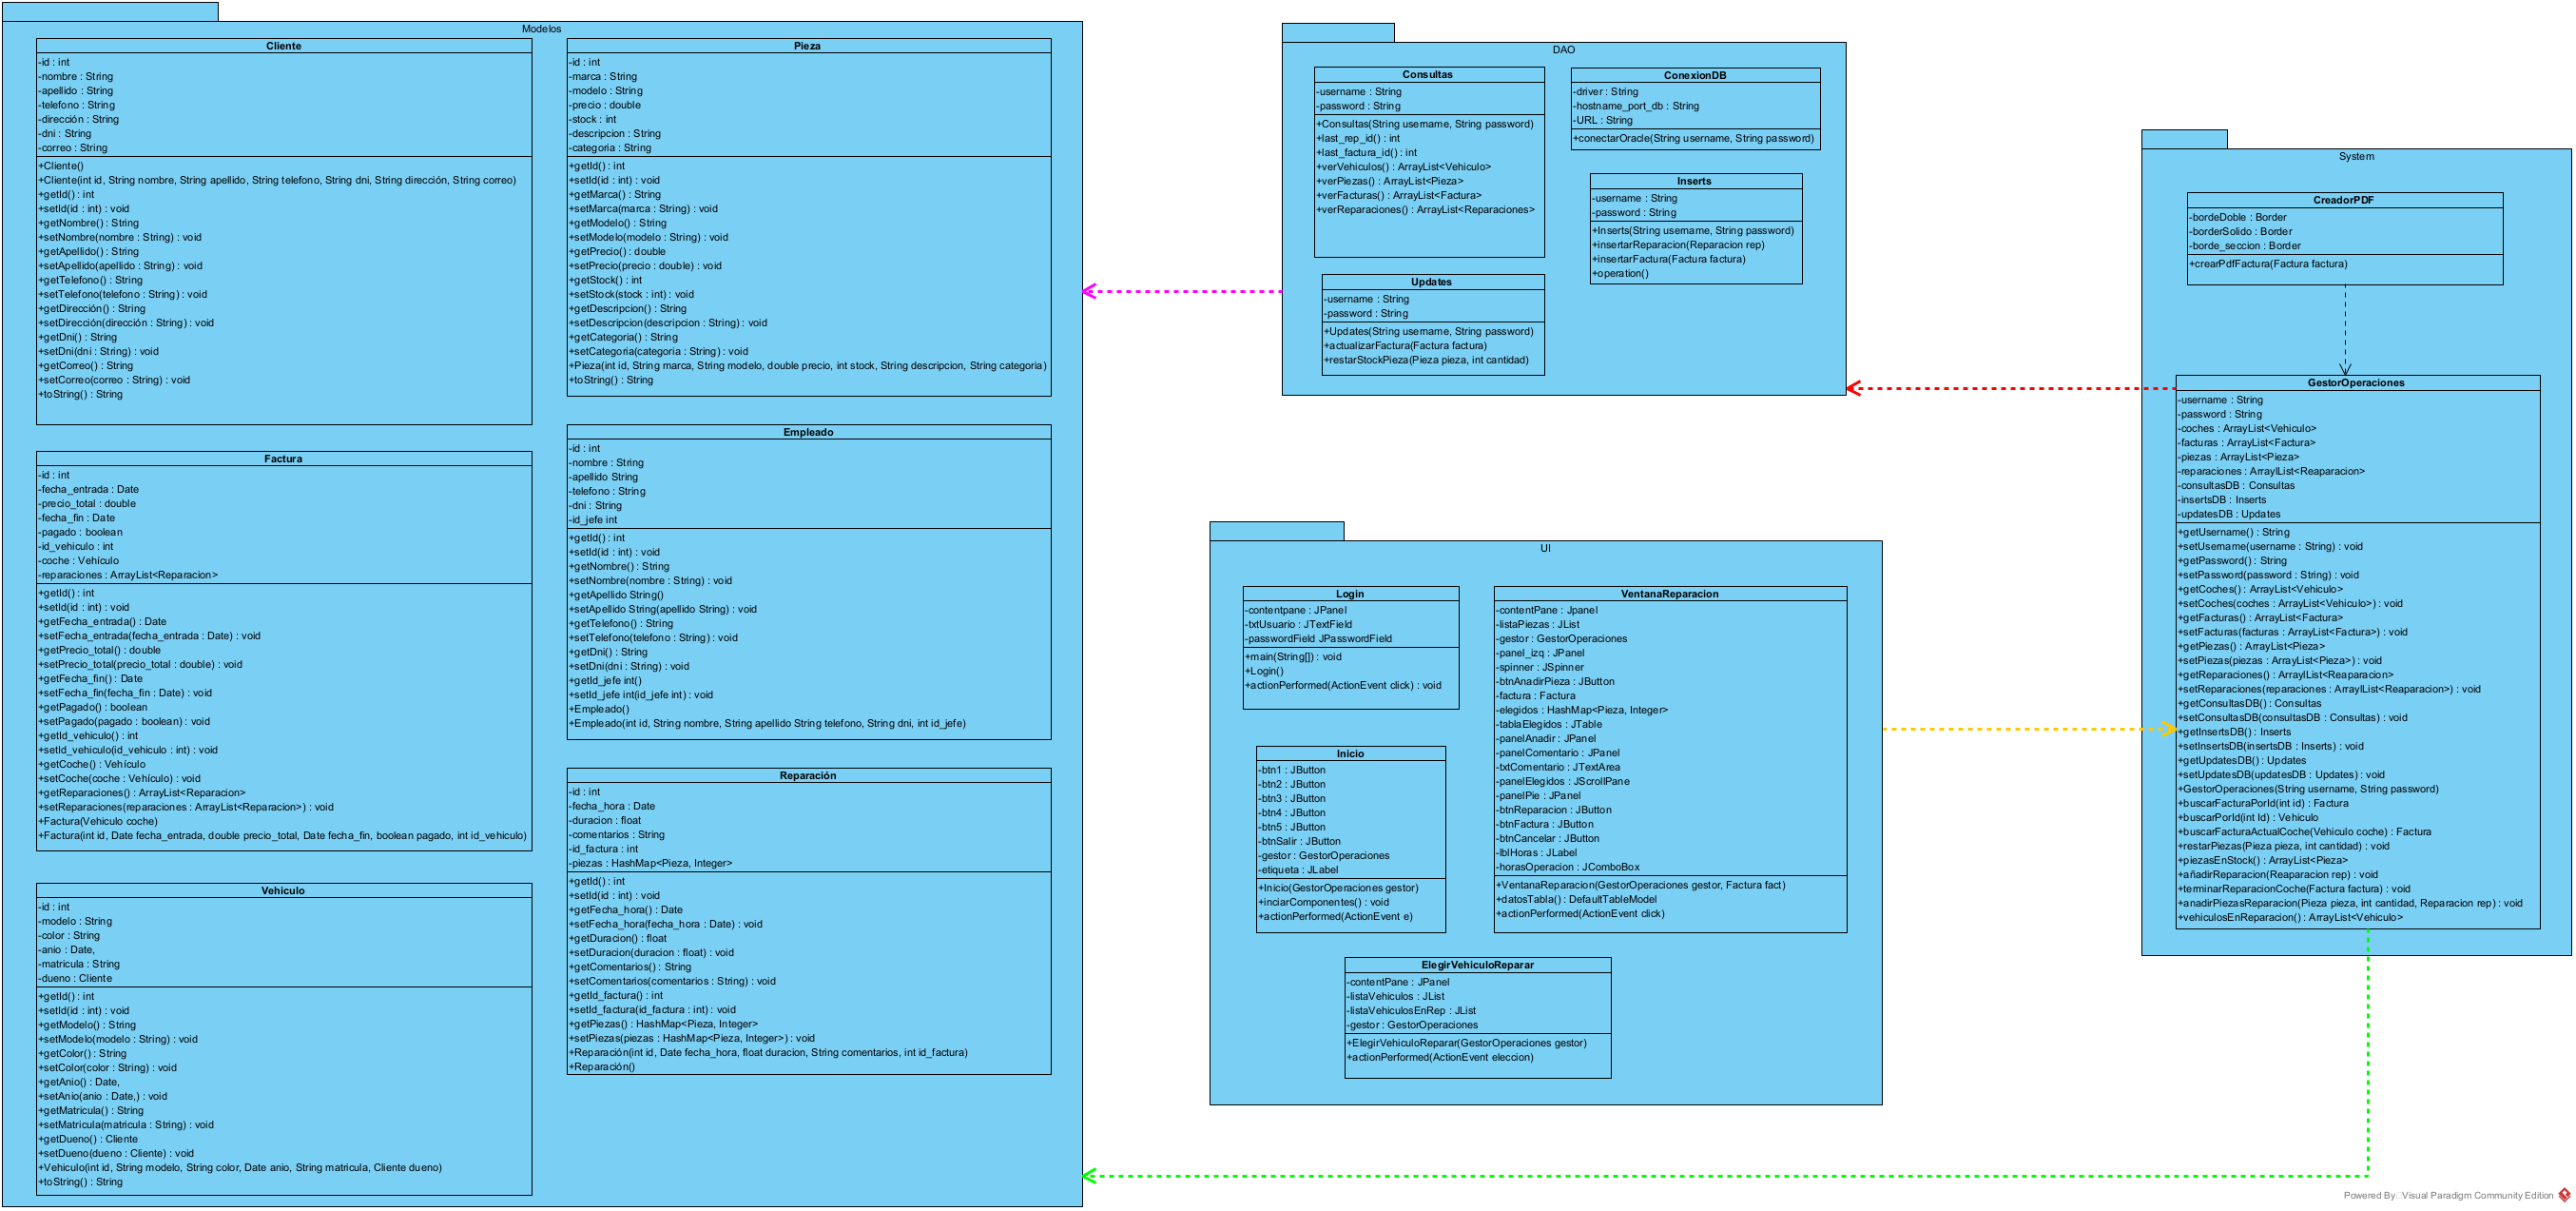
\includegraphics[width=1.0\textwidth]{program/DiagramaDeClasesTaller.png}
  \caption{Diagrama de clases del programa.}
\end{figure}
En cuanto el empleado elija reparar un vehículo, el programa completará el siguiente diagrama de secuencia:
\begin{figure}[H]
  \centering
  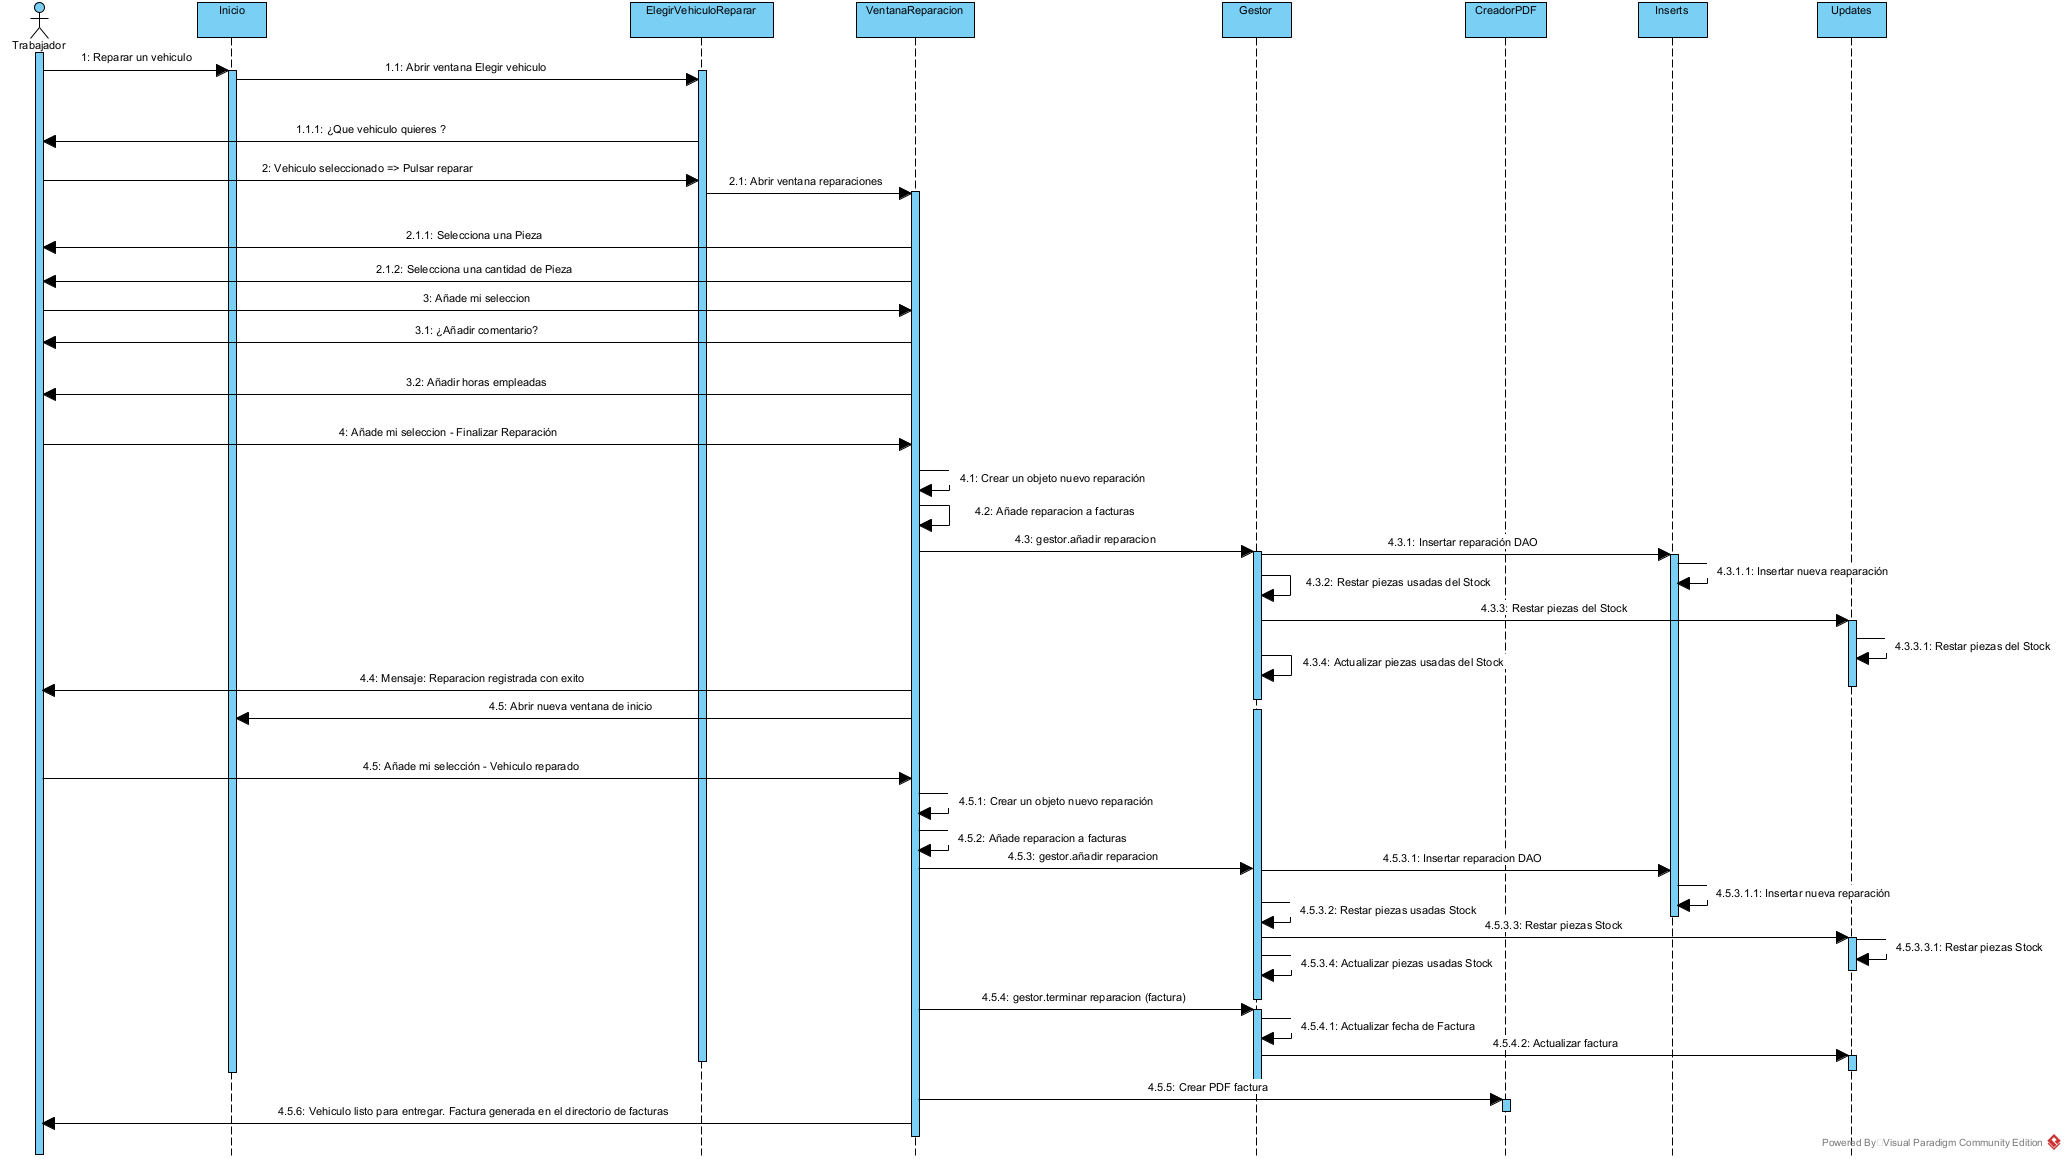
\includegraphics[width=1.0\textwidth]{program/SecuenciaRepararvehiculo.png}
  \caption{Secuencia al reparar un vehículo}
\end{figure}
\subsubsection{Esquema de red}
La conexión a internet se realizará via Wi-Fi, utilizando el Wi-Fi emitido por el router que estará en la oficina. Hemos optado 
por no utilizar cableado ya que creemos que hoy en día el Wi-Fi aporta suficiente fiabilidad y añadir cableado al taller podría provocar molestias a los empleados a la hora de utilizar 
maquinaría pesada y mover piezas por el taller.\\ 
El esquema de red es el siguiente: 
\begin{figure}[H]
  \centering
  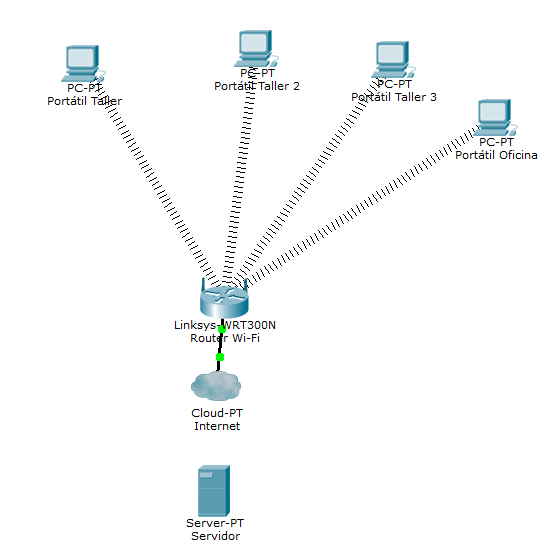
\includegraphics[width=1.0\textwidth]{CapturasSistemas/EsquemaRed.png}
  \caption{Esquema de Red propuesto.}
\end{figure}
\subsection{Planificación semanal}
\subsection{FOL}
\clearpage
\section{FASE 2: IMPLEMENTACIÓN Y PRUEBAS}
{
  \lstset{%
  	backgroundcolor=\color{white},
      inputencoding=utf8,
    escapeinside={\%*}{*)},
    literate={á}{{\'a}}1 {é}{{\'e}}1 {í}{{\'i}}1 {ó}{{\'o}}1 {ú}{{\'u}}1 {Á}{{\'A}}1 {É}{{\'E}}1 {Í}{{\'I}}1 {Ó}{{\'O}}1 {Ú}{{\'U}}1 {ñ}{{\~n}}1 {Ñ}{{\~N}}1,
  	basicstyle=\footnotesize,
  	breakatwhitespace=false,
  	breaklines=true,
    nolol=true,
  	captionpos=b,
  	commentstyle=\color{dkgreen},
  	deletekeywords={...},
  	escapeinside={\%*}{*)},
  	extendedchars=true,
  	frame=single,
  	keepspaces=true,
  	keywordstyle=\color{blue},
  	language=SQL,
  	morekeywords={*,modify,MODIFY,...},
  	numbers=left,
  	numbersep=15pt,
  	numberstyle=\tiny,
  	rulecolor=\color{ltgray},
  	showspaces=false,
  	showstringspaces=false, 
  	showtabs=false,
  	stepnumber=1,
  	tabsize=3,
}
\subsection{DDBB: Código SQL}
Para ver la instalación de la SGDB de Oracle, referiros a la sección de Sistemas Informáticos, al apartado \ref{subsubsection:Software}. En este apartado nos limitaremos a describir el código sql ejecutado en la BD.\\
Para poner en marcha nuestra base de datos, primero hemos creado dos datafiles en los que se dividirá el contenido. \\ Luego hemos creado un usuario de jefe o administrador, y 5 cuentas para los mecánicos, y hemos modificado sus perfiles,
permitiendo tan solo 1 inicio de sesión simultaneo por usuario. También hemos creado un usuario para los visitantes de la web, este usuario tiene la posibilidad de crear sesiones simultaneas ilimitadas. \\ 
Luego hemos creado las tablas que podemos observar en la figura \ref{fig:ER} . Cabe destacar que para tener IDs autogenerados ascendentes, hemos utilizado la siguiente secuencia:\\
\begin{lstlisting}[caption=Código sql para autogenerar IDs]
  CREATE SEQUENCE CLIENTES_SEQ START WITH 1;

  CREATE OR REPLACE TRIGGER CLIENTES_IDS BEFORE INSERT ON CLIENTE FOR EACH ROW
  BEGIN SELECT CLIENTES_SEQ.NEXTVAL INTO :NEW.ID_CLIENTE FROM DUAL;
  END;
\end{lstlisting}
Después de crear las tablas hemos establecido las relaciones entre ellas y hemos añadido algún constraint como puede ser el formato de DNI de un cliente o el formato de un correo electrónico.\\ 
Hemos limitado los permisos que tienen los mecánicos en las tablas, ya que en nuestro diseño no deben ser capaces de modificar algunos parámetros como pueden ser los precios de las piezas. También hemos concedido permiso para
realizar select en las tablas de piezas y categorías al usuario de la web, ya que son las únicas tablas que debe ver, y en ningún caso editar.\\ 
Finalmente, hemos insertado datos de prueba en todas las tablas para comprobar la correcta creación de estas y tener una base sobre la que trabajar.\\ 
Todas las ordenes sql realizadas están en el script disponible en el \href{https://github.com/DreaMan92/TrabajoTaller/blob/main/BBDD/Oracle/Script.sql}{\color{red}{repositorio de github}}.
}

\subsection{Programación: Clases y métodos}
  \subsubsection{Organización del Código}
  En nuestro programa hemos decidido separar la lógica de negocio de las interfaces.\\ 
  Hemos dividido las clases en 4 paquetes:\\
  \begin{itemize}
    \item Modelos: En este paquete están las clases que representan las entidades del negocio. 
    \item DAO: En este paquete están las clases que se encargan de realizar la conexión con la base de datos, y realizar las querys necesarias.
    \item System: En este paquete están las clases que contienen los metodos que realizan las acciones relacionadas con el negocio, como buscar una factura concreta o crear una reparacion. En este paquete hemos creado una clase llamada CreadorPDF 
    que hace uso de la librería \href{https://github.com/itext}{\color{red}{iText}} para crear una factura en formato .pdf.
    \item UI: En este paquete están las interfaces gráficas con sus controladores. 
  \end{itemize}
  El código fuente de todo el programa se puede ver en el \href{https://github.com/martinfgar/TallerProgramacion}{\color{red}{repositorio de github del proyecto}}.
  \subsubsection{Capturas de Ejecución}
  En las siguientes capturas podemos ver la ejecución del programa:\\
  \begin{figure}[H]
    \centering
    \begin{subfigure}{.5\textwidth}
      \centering
      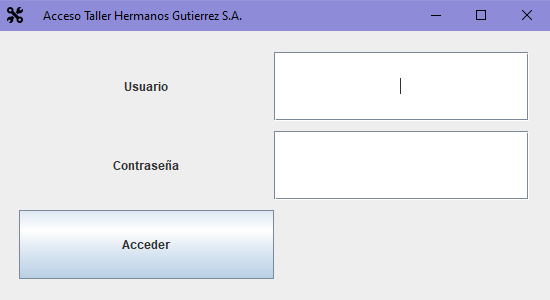
\includegraphics[width=0.9\linewidth]{program/capturasEjec/login.PNG}
      \caption{Pantalla de Login de AppTaller.}
    \end{subfigure}%
    \begin{subfigure}{.5\textwidth}
      \centering
      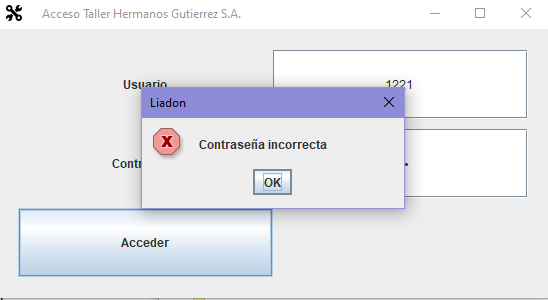
\includegraphics[width=0.9\linewidth]{program/capturasEjec/loginFallido.PNG}
      \caption{Login fallido.}
    \end{subfigure}
    \caption{Pantalla Login.}
  \end{figure}
  El login de nuestro programa funciona en conjunto con el de la base de datos, es decir, utiliza los mismos usuarios y contraseñas. Por lo tanto, si el programa no es capaz de alcanzar la base de datos,
  no se podrá utilizar.\\

    \begin{figure}[H]
      \centering
      \begin{subfigure}{.5\textwidth}
        \centering
        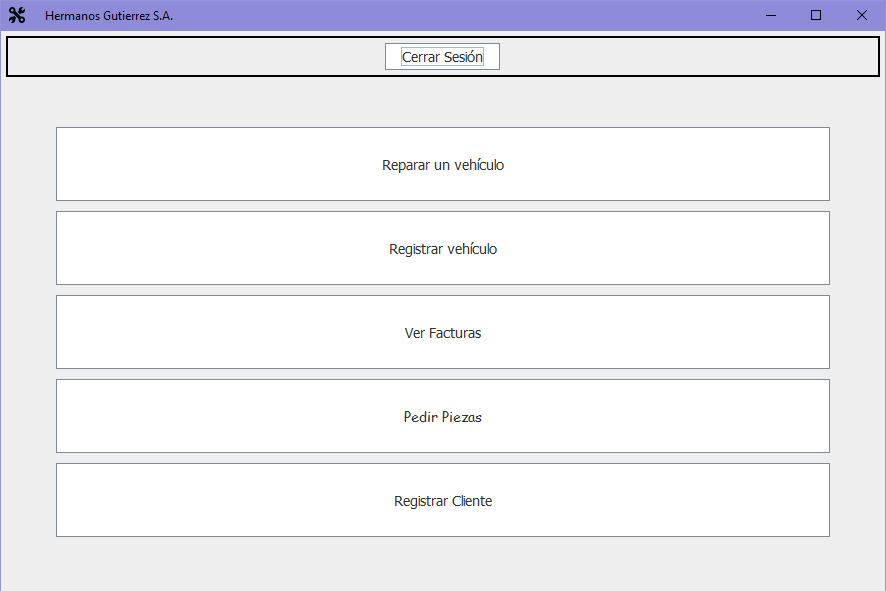
\includegraphics[width=0.9\linewidth]{program/capturasEjec/menu.PNG}
        \caption{Pantalla menu de opciones una vez logueado.}
      \end{subfigure}%
      \begin{subfigure}{.5\textwidth}
        \centering
        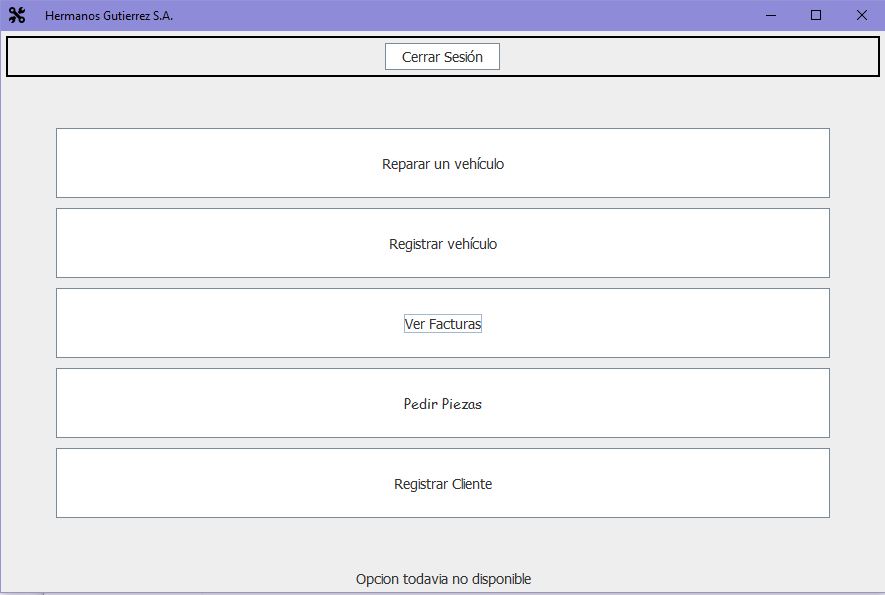
\includegraphics[width=0.9\linewidth]{program/capturasEjec/menuNoOption.PNG}
        \caption{Al elegir una opcion que no desarrollada.}
      \end{subfigure}
      \caption{Pantalla Menu.}
    \end{figure}
  En nuestro programa solo funciona la opción de reparar vehículo, ya que hemos acordado que será la única que implementaremos. Al elegir la opción de reparar vehículo se nos muestra la siguiente pantalla. 
  Cuando a algún vehículo se le ha realizado alguna reparación pero aún no se ha terminado con él, está pantalla lo mostrará en la lista de la derecha:\\
  \begin{figure}[H]
    \centering
    \begin{subfigure}{.5\textwidth}
      \centering
      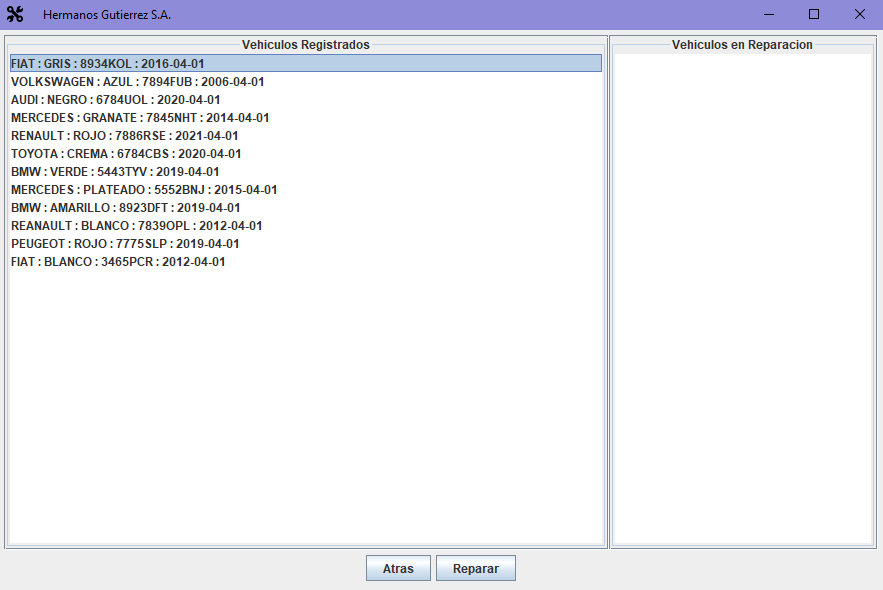
\includegraphics[width=0.9\linewidth]{program/capturasEjec/menuElegirVehiculo.PNG}
      \caption{Menu para elegir vehículo cuando no hay ninguna reparación comenzada.}
    \end{subfigure}%
    \begin{subfigure}{.5\textwidth}
      \centering
      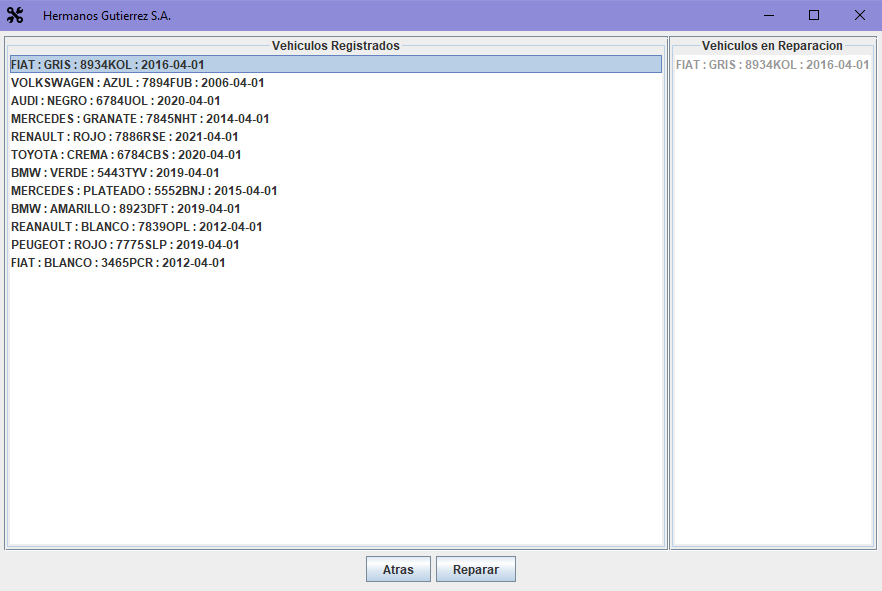
\includegraphics[width=0.9\linewidth]{program/capturasEjec/menuElegirVehiculo2.PNG}
      \caption{Menu para elegir vehículo cuando hay una reparación comenzada.}
    \end{subfigure}
    \caption{Pantalla Elegir Vehiculo.}
  \end{figure}

  Finalmente, la pantalla de reparación tiene dos opciones para finalizar: Finalizar reparación y vehículo preparado. Con el primero finalizamos la tarea, pero el vehículo aún tiene
  operaciones pendientes, con lo que no está preparado para ser entregado. Con el segundo dejamos el vehículo preparado para su recogida y se genera una factura en pdf. 
  \begin{figure}[H]
    \centering
    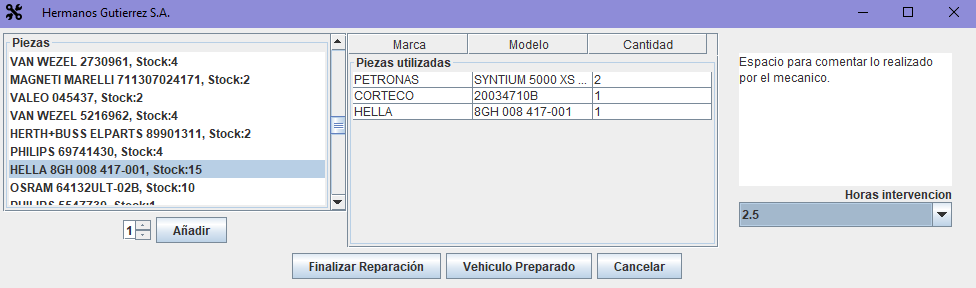
\includegraphics[width=1.0\textwidth]{program/capturasEjec/reparacion.PNG}
    \caption{Pantalla Reparación.}
  \end{figure}
  \begin{figure}[H]
    \centering
    \begin{subfigure}{.5\textwidth}
      \centering
      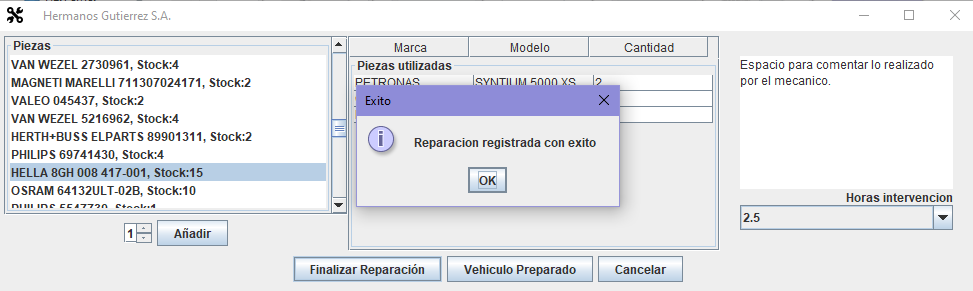
\includegraphics[width=0.9\linewidth]{program/capturasEjec/reparacion2.PNG}
      \caption{Opción finalizar reparación.}
    \end{subfigure}%
    \begin{subfigure}{.5\textwidth}
      \centering
      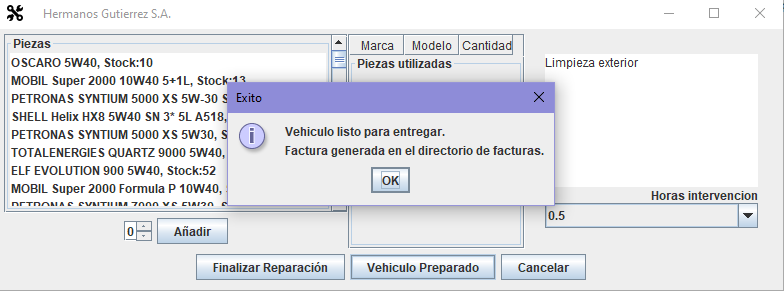
\includegraphics[width=0.9\linewidth]{program/capturasEjec/reparacion3.PNG}
      \caption{Opción vehículo preparado}
    \end{subfigure}
    \caption{Pantalla Reparación, dos opciones.}
  \end{figure}
  Tras finalizar de reparar un vehículo, se genera una factura con la información relevante: 
  \begin{figure}[H]
    \centering
    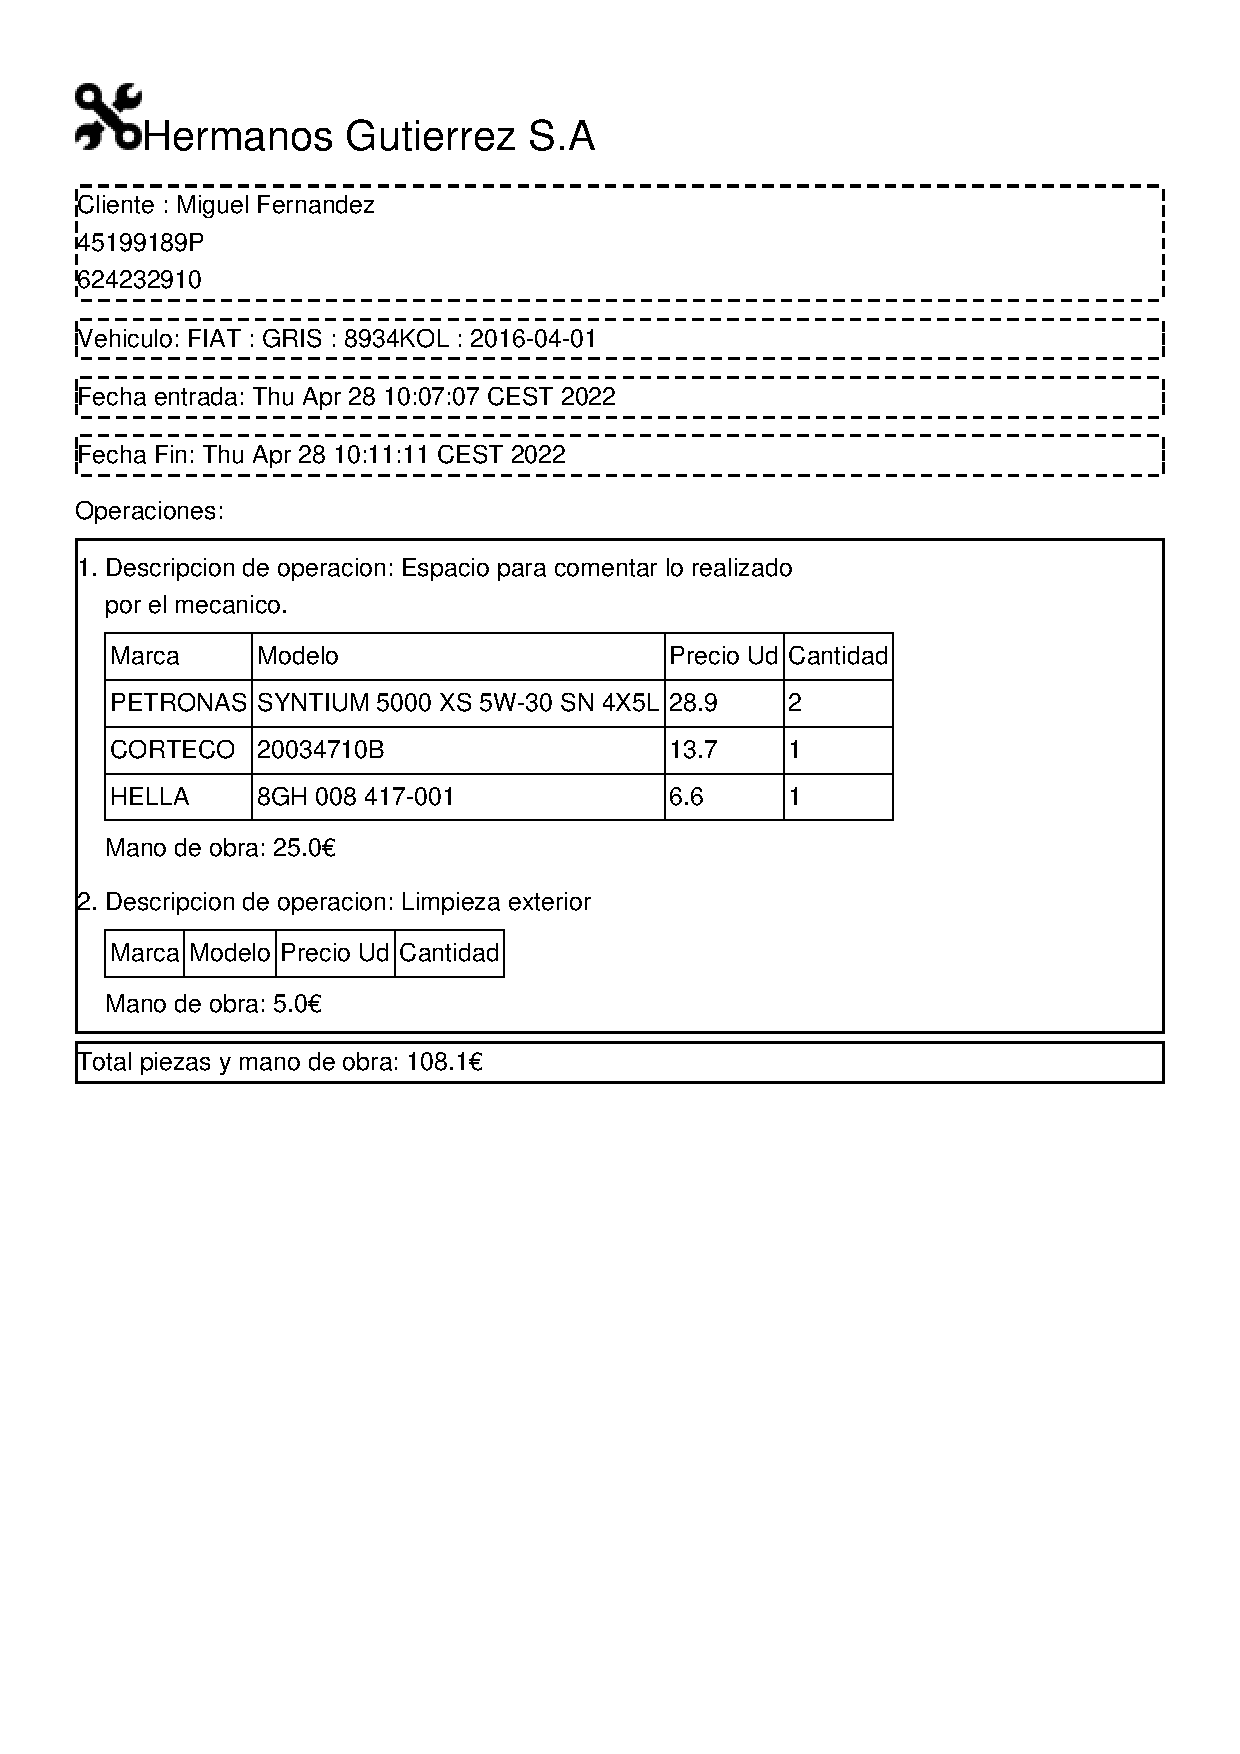
\includegraphics[width=1.0\textwidth]{program/capturasEjec/Factura 6.pdf}
    \caption{Factura generada.}
  \end{figure}

\subsection{Lenguaje de Marcas: conjunto de ficheros}
La página web consta de 4 páginas estáticas, y otras 2 plantillas que se renderizan en el servidor.\\
Para el renderizado de estas páginas utilizamos \href{https://www.thymeleaf.org/}{\color{red}{Thymeleaf}}, junto al backend programado en Java utilizando Spring.\\
Todo el código fuente se puede consultar en el \href{https://github.com/martinfgar/WebTaller}{\color{red}{repositorio del proyecto}}.
\subsubsection{Páginas estáticas}
\paragraph{index.html}
\begin{figure}[H]
  \centering
  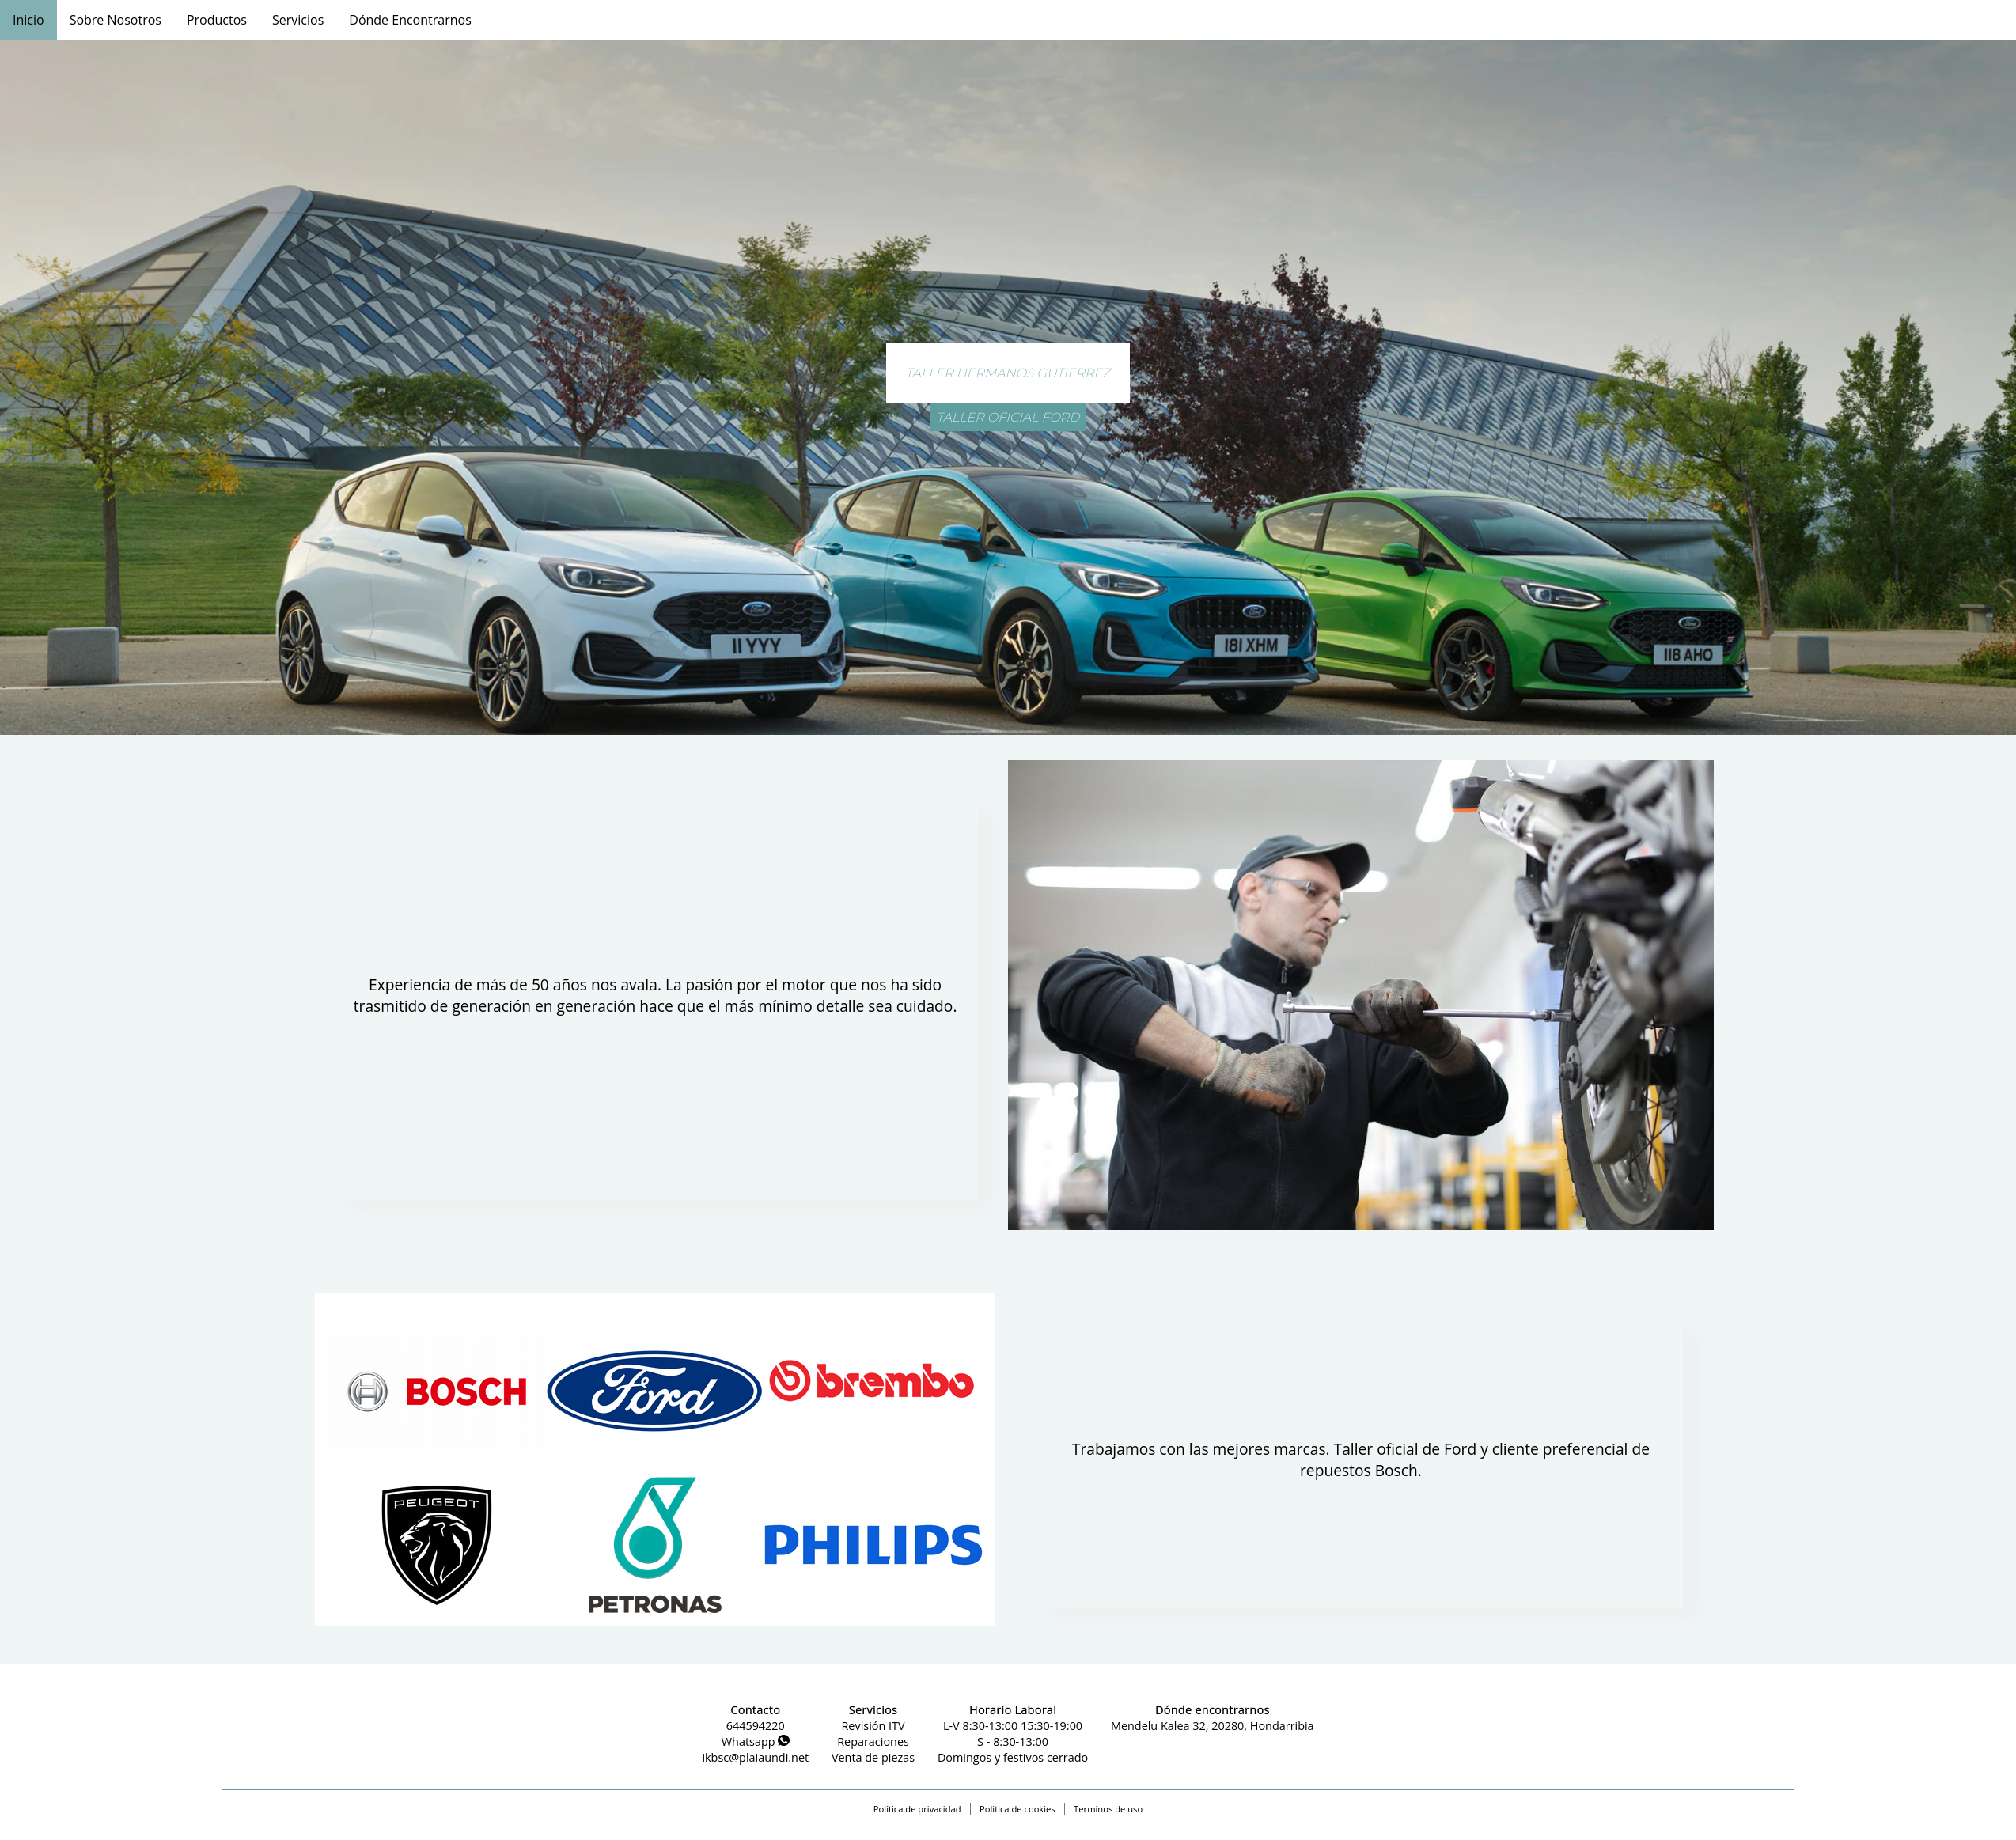
\includegraphics[width=1.0\textwidth]{LMSI/CapturasWeb/index.png}
  \caption{index.html}
\end{figure}
\paragraph{location.html}
\begin{figure}[H]
  \centering
  \includegraphics[width=1.0\textwidth]{LMSI/CapturasWeb/dondeEncontrarnos.png}
  \caption{location.html}
\end{figure}
\paragraph{mecanicos.html}
\begin{figure}[H]
  \centering
  \includegraphics[width=0.7\textwidth]{LMSI/CapturasWeb/SobreNosotros.png}
  \caption{mecanicos.html}
\end{figure}
Para rellenar el contenido de esta página, hemos creado un script de JavaScript que
obtiene el fichero mecanicos.xml, y utilizando su contenido modifica el código html.
{
  \lstset{language=XML,
  backgroundcolor=\color{white},
  inputencoding=utf8,
  escapeinside={\%*}{*)},
  literate={á}{{\'a}}1 {é}{{\'e}}1 {í}{{\'i}}1 {ó}{{\'o}}1 {ú}{{\'u}}1 {Á}{{\'A}}1 {É}{{\'E}}1 {Í}{{\'I}}1 {Ó}{{\'O}}1 {Ú}{{\'U}}1 {ñ}{{\~n}}1 {Ñ}{{\~N}}1,
  breakatwhitespace=false,
    showspaces=false,
    showtabs=false,
    breaklines=true,
    showstringspaces=false,
    breakatwhitespace=true,
    captionpos=b,
    frame=single,
    basicstyle=\ttfamily,
    moredelim=[il][\textcolor{pgrey}]{$$},
    moredelim=[is][\textcolor{pgrey}]{\%\%}{\%\%}
  }
    \begin{lstlisting}[caption=mecanicos.xml]
      <?xml version="1.0" encoding="UTF-8"?>
      
      <empleados xmlns:xsi="http://www.w3.org/2001/XMLSchema-instance" xsi:noNamespaceSchemaLocation="mecanicos.xsd">
          <empleado>
              <imagen>"imagenes/juanRodriguez.jpg"</imagen>
              <nombre>Juan Rodriguez</nombre>
              <descripcion>Ex-piloto de rally, apasionado del motor. Tras compartir experiencias con mecánicos y pilotos de todo
                  el mundo, se unió a nuestro equipo en 2015.</descripcion>
          </empleado>
          <empleado>
              <imagen>"imagenes/raulIruretagollena.jpg"</imagen>
              <nombre>Raul Iruretagollena</nombre>
              <descripcion>Desde 2018 en la empresa. Sus conocimientos sobre frenos podrían parar un tren.</descripcion>
          </empleado>
          <empleado>
              <imagen>"imagenes/juanjoUriburu.jpg"</imagen>
              <nombre>Juanjo Uriburu</nombre>
              <descripcion>Uno de los veteranos de la empresa, en la cual lleva desde 2002. Experto en escape de gases y
                  emisiones, se asegura de que con tu vehículo no contamines ni un gramo de más nuestro mundo.</descripcion>
          </empleado>
          <empleado>
              <imagen>"imagenes/soniaVirasoro.jpg"</imagen>
              <nombre>Sonia Virasoro</nombre>
              <descripcion>La experta en eléctricidad y electrónica, una profesional muy detallista que hace que todos los
                  pequeños detalles y funciones de tu vehículo no fallen nunca. Desde 2012 en Hermanos Gutierrez.</descripcion>
          </empleado>
          <empleado>
              <imagen>"imagenes/aitorSegurola.jpg"</imagen>
              <nombre>Aitor Segurola</nombre>
              <descripcion>Nuestro experto en transmisiones y suspensiones, se encarga de que tu vehículo funcione tan suave y
                  sea tan preciso como el primer día. Con nosotros desde 2014.</descripcion>
          </empleado>
          <empleado>
              <imagen>"imagenes/juanmariGutierrez.jpg"</imagen>
              <nombre>Juanmari Gutierrez</nombre>
              <descripcion>Hijo del co-fundador Eustaquio Gutierrez, tomo cargo de la empresa en 2008. Experto en motores y
                  combustión, sería capaz de encajar un motor de avión en un turismo.</descripcion>
          </empleado>
          
      </empleados>
      \end{lstlisting}
}
El script de JavaScript que dibuja este contenido es el siguiente:
{
  \definecolor{lightgray}{rgb}{.9,.9,.9}
  \definecolor{darkgray}{rgb}{.4,.4,.4}
  \definecolor{purple}{rgb}{0.65, 0.12, 0.82}
  \lstdefinelanguage{JavaScript}{
  keywords={typeof, new, true, false, catch, function, return, null, catch, switch, var, if, in, while, do, else, case, break},
  keywordstyle=\color{blue}\bfseries,
  ndkeywords={class, export, boolean, throw, implements, import, this},
  ndkeywordstyle=\color{darkgray}\bfseries,
  identifierstyle=\color{black},
  sensitive=false,
  comment=[l]{//},
  morecomment=[s]{/*}{*/},
  commentstyle=\color{purple}\ttfamily,
  stringstyle=\color{red}\ttfamily,
  morestring=[b]',
  morestring=[b]"
  }
  \lstset{
   language=JavaScript,
   backgroundcolor=\color{lightgray},
   extendedchars=true,
   basicstyle=\footnotesize\ttfamily,
   showstringspaces=false,
   showspaces=false,
   numbers=left,
   numberstyle=\footnotesize,
   numbersep=9pt,
   tabsize=2,
   breaklines=true,
   showtabs=false,
   captionpos=b
  }
  \begin{lstlisting}[caption=mecanicos.js]
window.addEventListener("load", function() {
	getRows();
});
function getRows() {
	var xmlhttp = new XMLHttpRequest();
	xmlhttp.open("get", "mecanicos.xml", true);
	xmlhttp.onreadystatechange = function() {
		if (this.readyState == 4 && this.status == 200) {
			showResult(this);
		}
	};
	xmlhttp.send(null);
}
function showResult(xmlhttp) {
    var xmlDoc = xmlhttp.responseXML.documentElement;
    var rowData = xmlDoc.getElementsByTagName("empleado");
    var wrapper = document.getElementById("mecanicos");
    console.log(rowData.length);
    for (i=0; i<rowData.length;i++){
        
        var url,name,desc;
        url = rowData[i].getElementsByTagName("imagen")[0].childNodes[0].nodeValue;
        console.log(url);
        name = rowData[i].getElementsByTagName("nombre")[0].childNodes[0].nodeValue;
        desc = rowData[i].getElementsByTagName("descripcion")[0].childNodes[0].nodeValue;
        if (i%2 == 0){
            imagenIzq(wrapper,url,name,desc);
        } else {
            imagenDer(wrapper,url,name,desc);
        }
    }
}



function imagenIzq(wrapper,url,name,desc){
    var texto = "<img src="+url+" alt=''><div class='info'><h6>"+name+"</h6><p>"+desc+"</p></div>";
    wrapper.insertAdjacentHTML("beforeend",texto)
}

function imagenDer(wrapper,url,name,desc){
    var texto = "<div class='info'><h6>"+name+"</h6><p>"+desc+"</p></div><img src="+url+" alt=''>";
    wrapper.insertAdjacentHTML("beforeend",texto)
}

  \end{lstlisting}
}
\paragraph{servicios.html}
\begin{figure}[H]
  \centering
  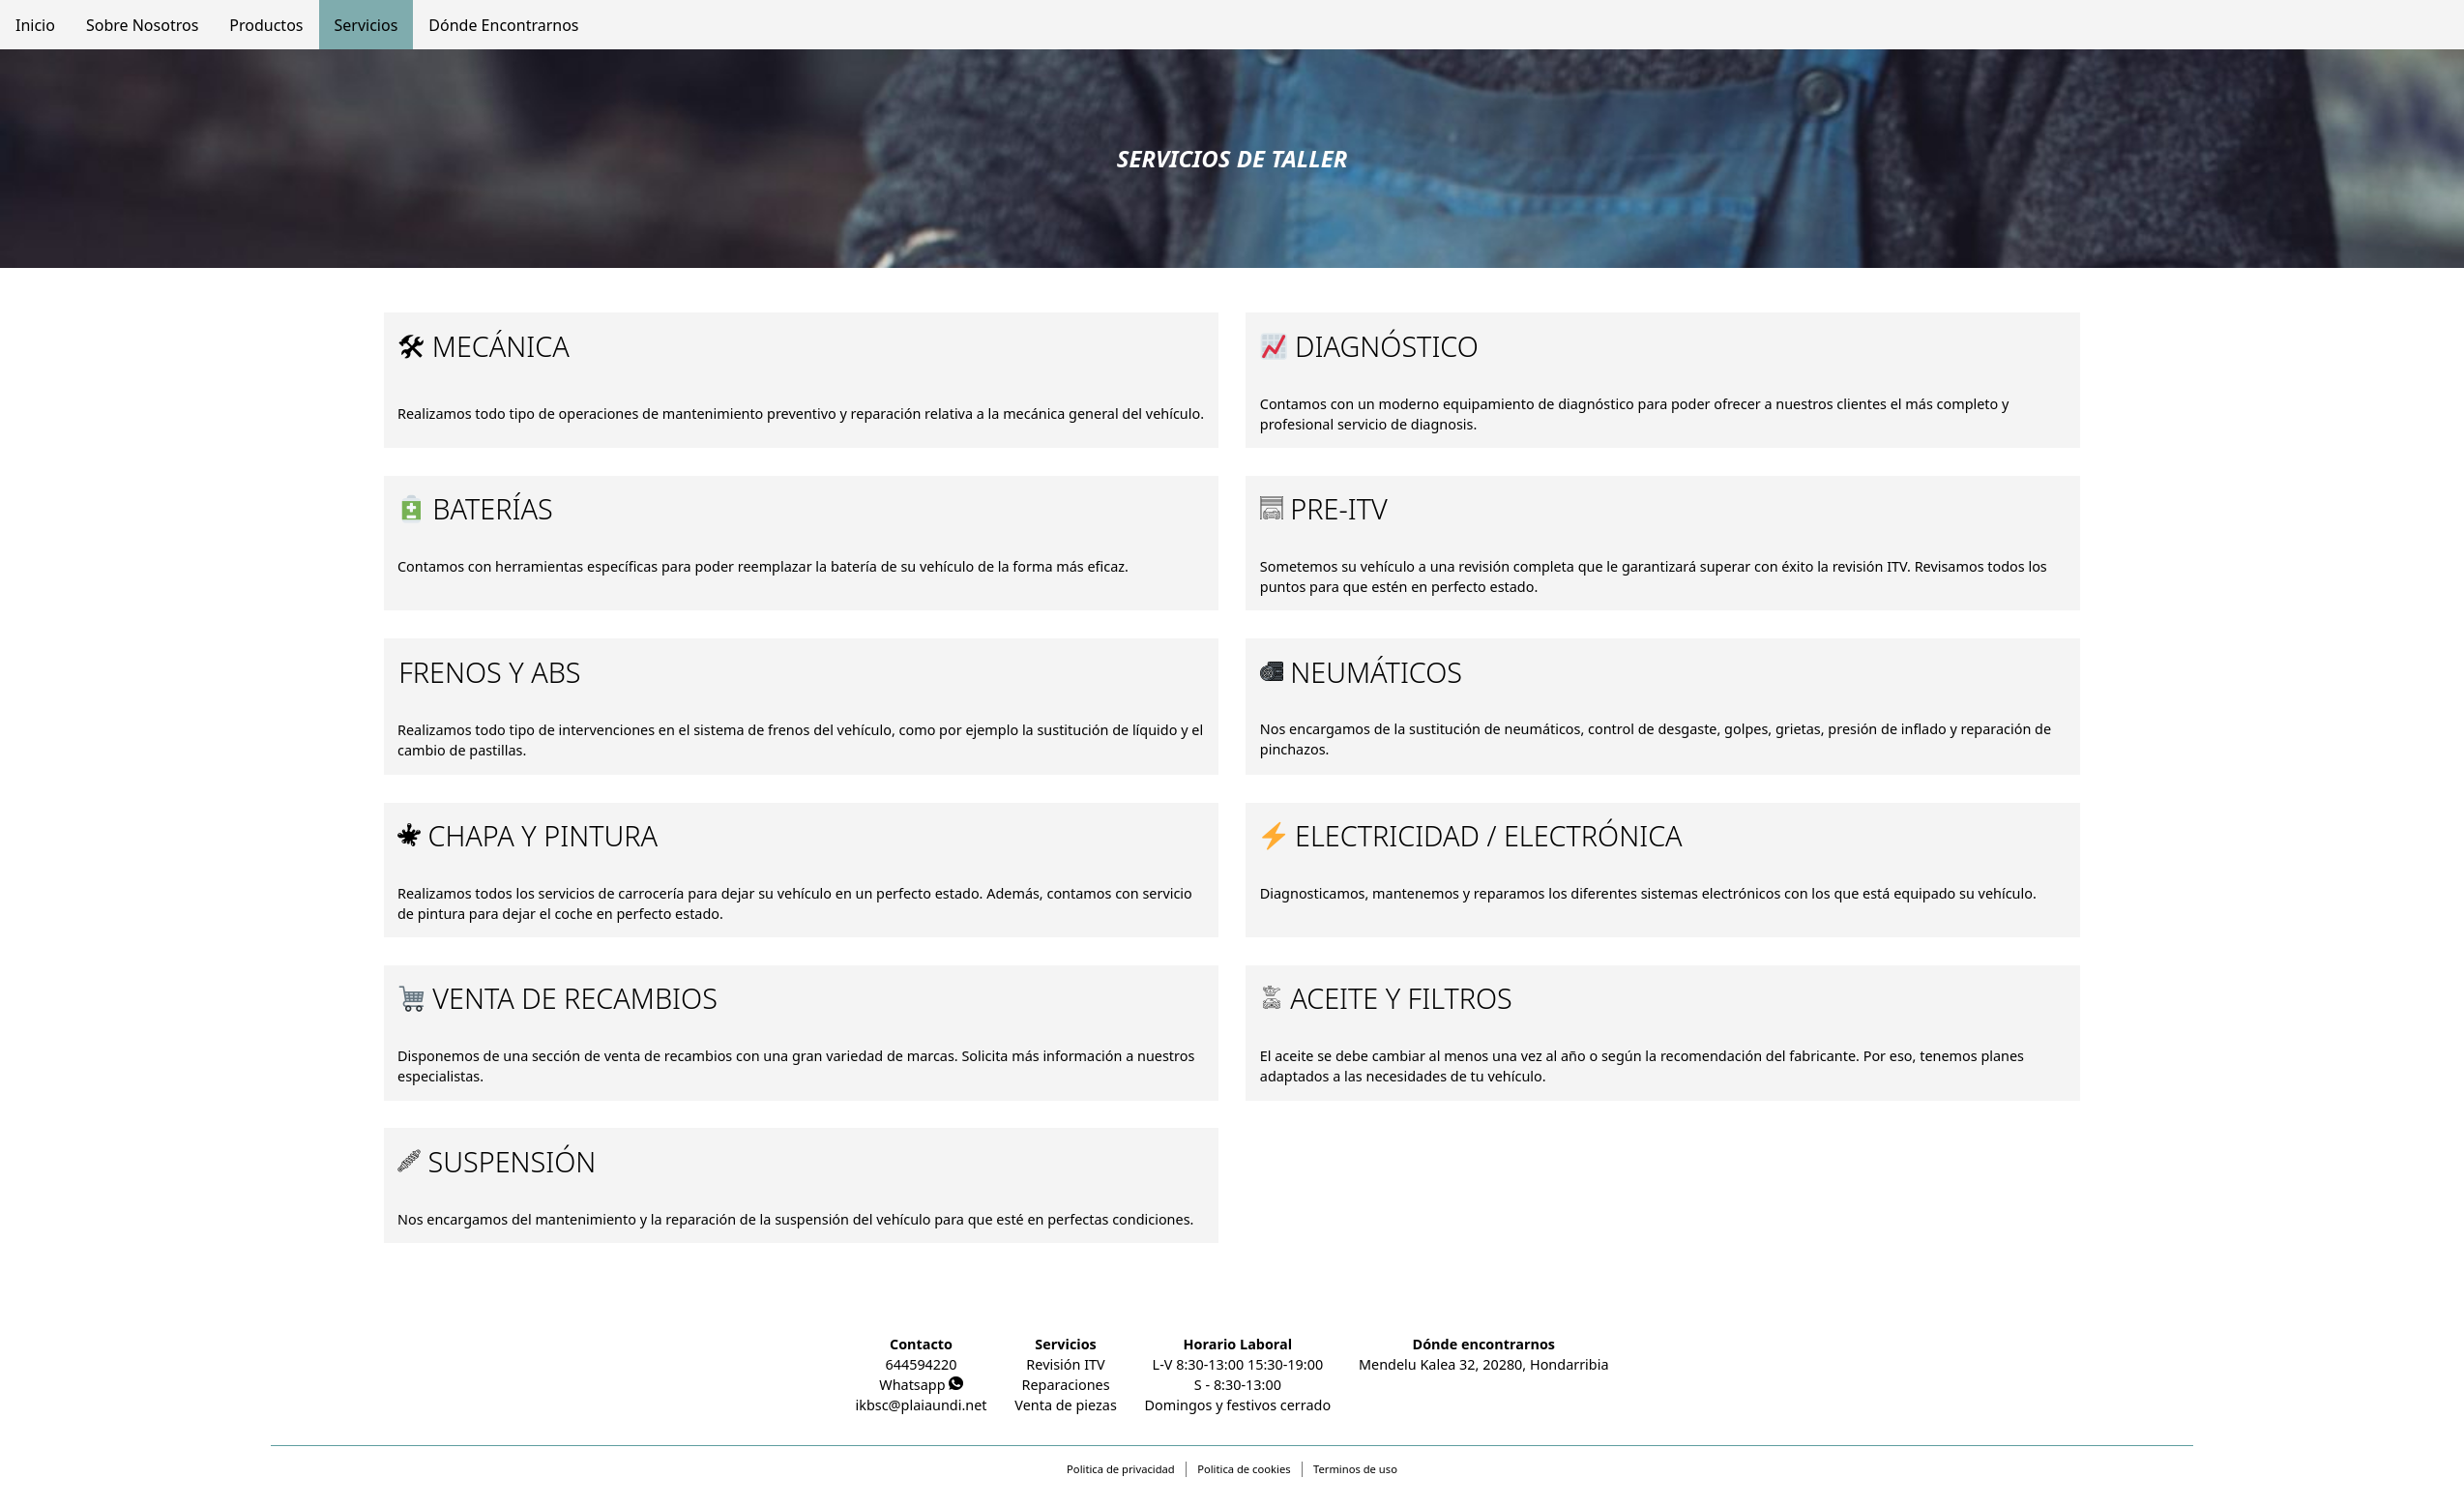
\includegraphics[width=1.0\textwidth]{LMSI/CapturasWeb/Servicios.png}
  \caption{servicios.html}
\end{figure}
\subsubsection{Páginas Dinamicas}

\paragraph{Productos.html}
\begin{figure}[H]
  \centering
  \includegraphics[width=1.0\textwidth]{LMSI/CapturasWeb/Productos.png}
  \caption{Productos.html}
\end{figure}
\begin{figure}[H]
  \centering
  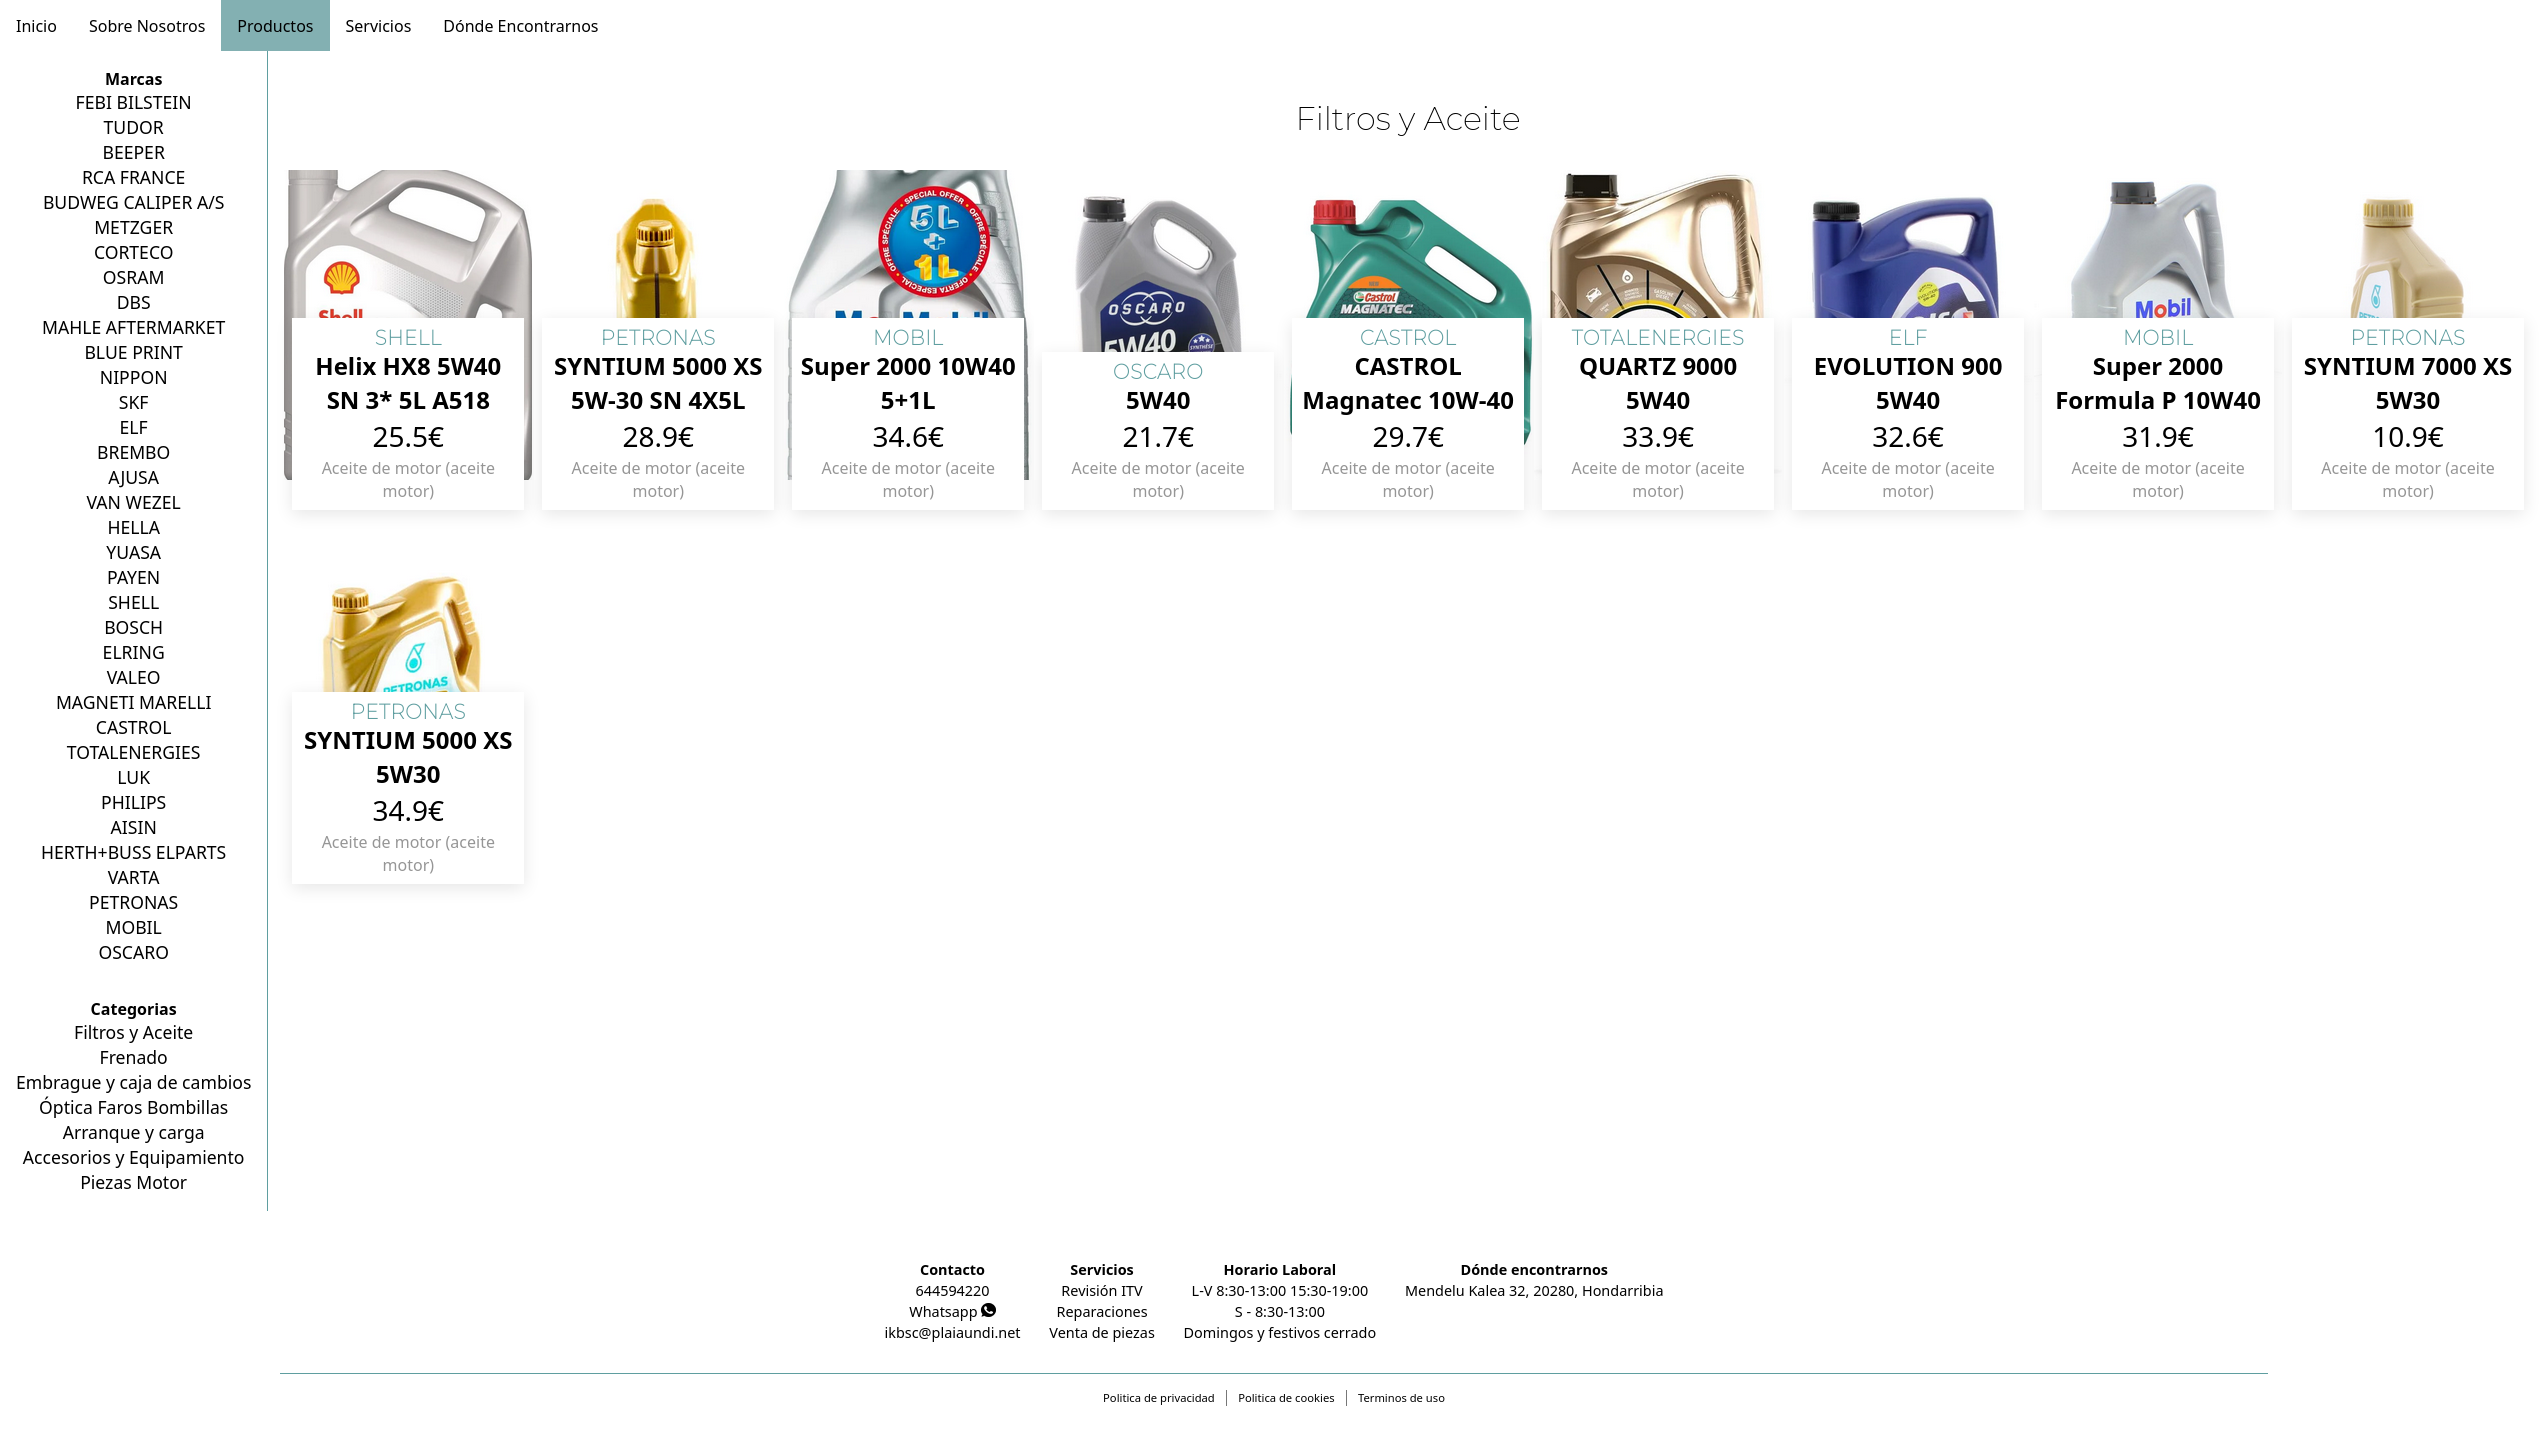
\includegraphics[width=1.0\textwidth]{LMSI/CapturasWeb/ProductosFiltrado.png}
  \caption{Productos.html según categoría}
\end{figure}
\paragraph{PaginaProducto.html}
\begin{figure}[H]
  \centering
  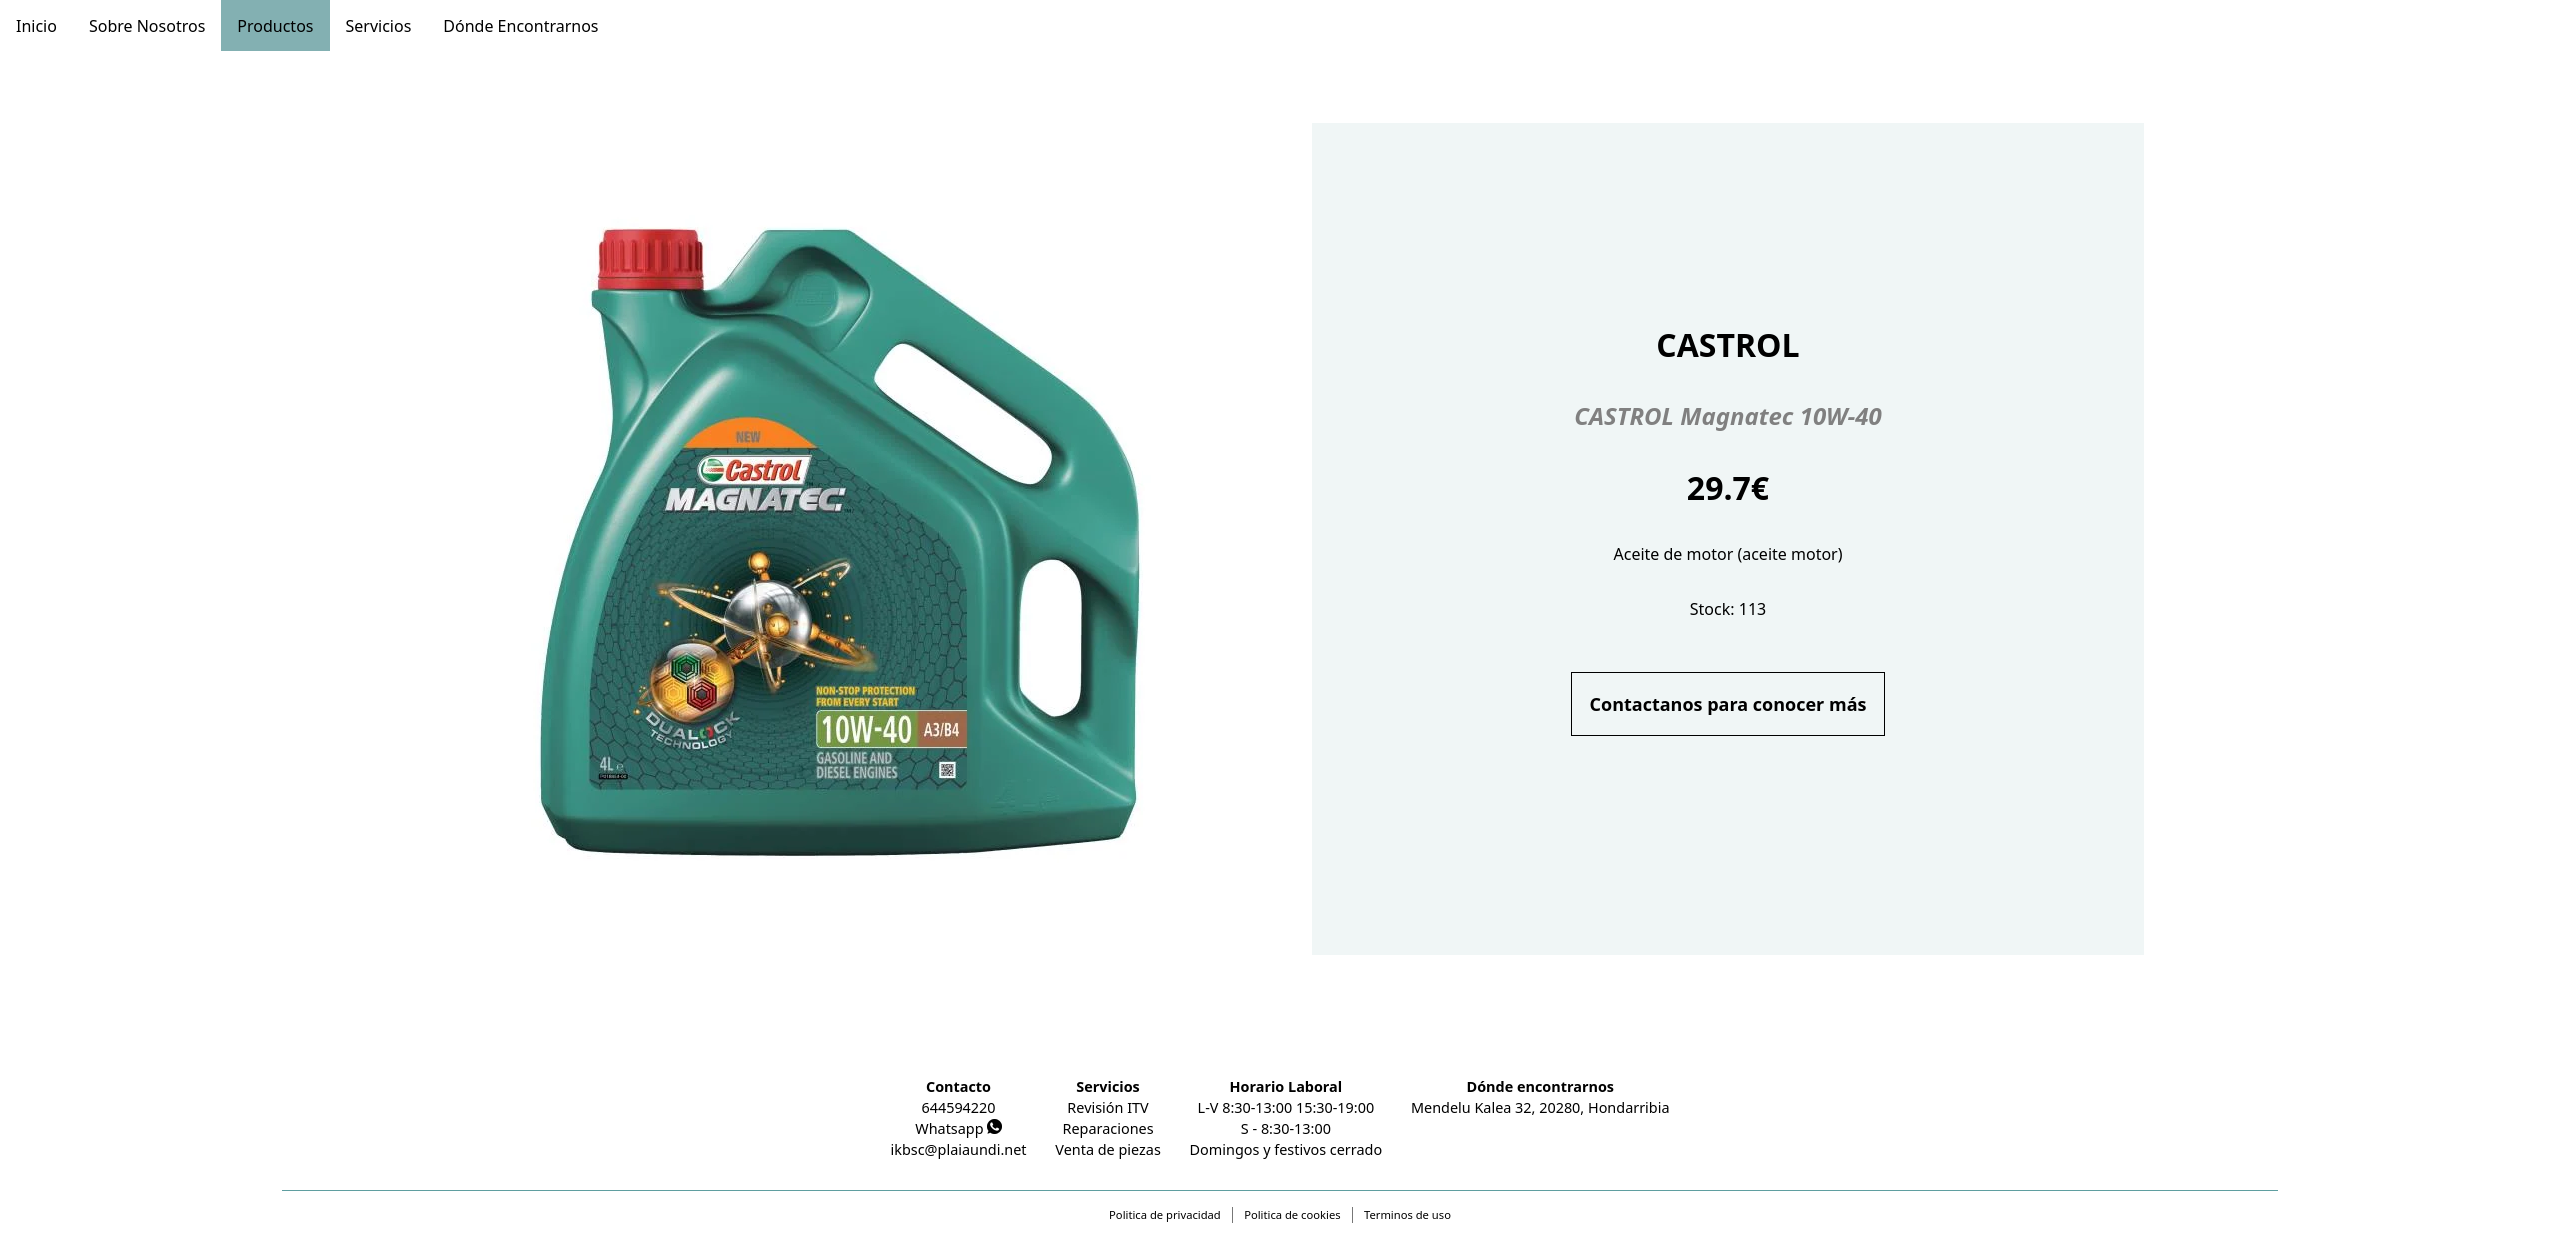
\includegraphics[width=1.0\textwidth]{LMSI/CapturasWeb/Producto.png}
  \caption{Producto.html}
\end{figure}
\subsubsection{CSS}
Todas estas páginas las hemos decorado utilizando CSS puro, sin utilizar ninguna librería como Bootstrap. Algunos ficheros .css son de uso común entre distintas páginas, ya que decoran la barra de navegación o el footer. \\
Los ficheros utilizados son:\\
\begin{itemize}
  \item nav.css
  \item footer.css
  \item general.css
  \item index.css
  \item mecanicos.css
  \item servicios.css
  \item location.css
  \item Productos.css
  \item tarjetaProducto.css
  \item PaginaProducto.css
\end{itemize}
\subsubsection{Imagenes e Iconos}
Las imagenes utilizadas provienen de nuestro servidor (previamente obtenidas de la página de imagenes de uso libre \href{https://www.pexels.com/es-es/}{\color{red}{Pexels}}), salvo en el caso de las imagenes de los productos. En esos casos, las url provienen de la página web \href{https://www.oscaro.es/}{\color{red}{Oscaro}}, que a su vez utiliza imágenes cedidas por el fabricante.\\
En un caso de un taller real, contactariamos con los proveedores para hacer uso de imagenes que ellos dispongan, y almacenarlas en nuestro servidor.\\ 
\subsection{SSII: Instalación y configuración y puesta en marcha.} 
\label{subsection:Sistemas}
\subsubsection{Hardware}
En nuestro caso hemos optado por equipar el taller con 4 portátiles con el SO Windows. 1 de ellos estaría colocado en la oficina y será el portátil del administrador, los otros 3 estarán colocados 
en los puestos de reparación de vehículos del taller.\\
Debido a las limitadas necesidades que tendrán estos portátiles, hemos optado por el modelo \href{https://www.pccomponentes.com/acer-travelmate-p2-tmp214-53-37at-intel-core-i3-1115g4-8gb-256gb-ssd-14}{\color{red}{{Acer Travelmate P2}}}.\\
\begin{figure}[H]
  \centering
  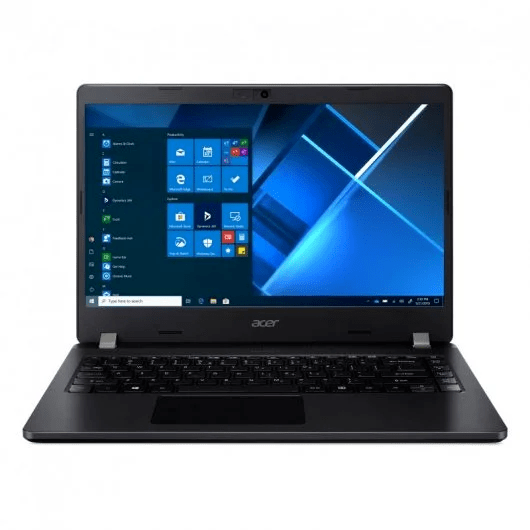
\includegraphics[width=0.6\textwidth]{CapturasSistemas/portatil.png}
  \caption{Portátil Acer Travelmate P2}
  \caption*{Fuente: \href{https://www.pccomponentes.com/acer-travelmate-p2-tmp214-53-37at-intel-core-i3-1115g4-8gb-256gb-ssd-14}{https://www.pccomponentes.com/}}
\end{figure}
\begin{itemize}
  \item Procesador: Intel Core i3-1115g4
  \item Memoria Ram: 8 GB DDR4
  \item Almacenamiento: 256 GB SSD PCIe
  \item Conectividad: \begin{itemize}
    \item Gigabit Ethernet
    \item Intel Wi-Fi 6 AX201 (802.11)
    \item Bluetooth
  \end{itemize}
  \item SO: Windows 10 Home 64 Bits
\end{itemize}
La base de datos y la página web la alojaremos en un VPS con una instalación del SO Ubuntu Server. En nuestro caso hemos optado por contratar el servidor \href{https://www.arsys.es/servidores/vps}{\color{red}{Arsys VPS M}},
ya que su centro de datos está en España, con lo que tendriamos una latencia más baja que con otras opciones. \\
Finalmente, para la línea telefónica y de internet hemos optado por contratar la operadora Guuk. Con una velocidad de 600mb simétricos, creemos que es suficiente para las necesidades del taller. \\

Presupuesto total de hardware/Software: \\
\begin{itemize}
  \item Portátiles: 1864.12€
  \item Servidor: 120€/Año
  \item Dominio: 15€/Año
  \item Internet: 504€/Año
\end{itemize}
\subsubsection{Software}
\label{subsubsection:Software}
{
En los portátiles con Windows 10, instalariamos el programa AppTaller creado por nosotros. No haría falta nada más para tener los ordenadores operativos. \\ 
\paragraph{Instalación SGDB}
Para poner en marcha la base de datos en el servidor, primero hemos instalado docker en el mismo. Para ello hemos ejecutado los siguientes comandos: 
  \lstset{%
  	backgroundcolor=\color{white},
    inputencoding=utf8,
    language=bash,
    escapeinside={\%*}{*)},
    literate={á}{{\'a}}1 {é}{{\'e}}1 {í}{{\'i}}1 {ó}{{\'o}}1 {ú}{{\'u}}1 {Á}{{\'A}}1 {É}{{\'E}}1 {Í}{{\'I}}1 {Ó}{{\'O}}1 {Ú}{{\'U}}1 {ñ}{{\~n}}1 {Ñ}{{\~N}}1,
  	basicstyle=\footnotesize,
  	breakatwhitespace=false,
  	breaklines=true,
    nolol=true,
  	captionpos=b,
  	commentstyle=\color{dkgreen},
  	deletekeywords={...},
  	escapeinside={\%*}{*)},
  	extendedchars=true,
  	frame=single,
  	keepspaces=true,
  	keywordstyle=\color{blue},
  	morekeywords={*,modify,MODIFY,...},
  	numbers=left,
  	numbersep=15pt,
  	numberstyle=\tiny,
  	rulecolor=\color{ltgray},
  	showspaces=false,
  	showstringspaces=false, 
  	showtabs=false,
  	stepnumber=1,
  	tabsize=3,
  }
  \begin{lstlisting}
    sudo curl -fsSL sudo curl -fsSL https://get.docker.com -o get-docker.sh
    sudo chmod +x get-docker.sh
    ./get-docker.sh
  \end{lstlisting}
  Despues hemos añadido el usuario al grupo de docker, hemos creado los directorios donde se guardarán 
  los datos, y hemos creado el contenedor que tendrá la SGDB.
  \begin{lstlisting}
    sudo usermod -aG docker 1daw3
    mkdir Oracle
    cd Oracle 
    mkdir data 
    docker pull epiclabs/docker-oracle-xe-11g
    sudo docker run -d -v /home/1daw3/Oracle/data:/u01/app/oracle --name=TallerDB -p 1521:1521 --restart unless-stopped -e ORACLE_ALLOW_REMOTE=true -e ORACLE_PASSWORD=1daw3 epiclabs/docker-oracle-xe-11g
  \end{lstlisting}
  Hemos comprobado que el contenedor está en marcha con el siguiente comando: 
  \begin{figure}[H]
    \centering
    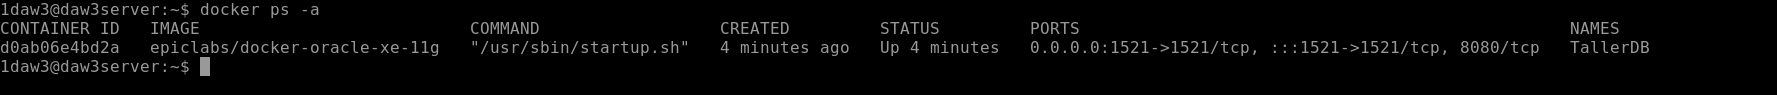
\includegraphics[width=1.0\textwidth]{CapturasSistemas/oracleEnMarcha.PNG}
    \caption{Comprobación de que el SGDB está en marcha.}
  \end{figure}
  \paragraph{Instalación Página/Servidor Web}
  En nuestro caso, hemos creado una aplicacion java (.jar) que contiene un servidor web Apache Tomcat incrustado. Esta 
  aplicación sirve el contenido HTML y CSS a traves del puerto 80. Hemos decidido crear un servicio de systemd para tener 
  el programa ejecutando en todo momento. Para ello hemos ejecutado los siguientes comandos: 
  \begin{lstlisting}
    sudo systemctl set-timezone Europe/Madrid
  \end{lstlisting}
  Con este comando hemos establecido el huso horario del servidor.
  Luego hemos creado el fichero \path{/etc/systemd/system/paginaWeb.service} con el siguiente contenido: 
  \begin{lstlisting}
    [Unit]
    Description=PaginaWebTaller
    After=syslog.target

    [Service]
    User=root
    ExecStart=/usr/bin/java -jar /home/1daw3/WebTaller-0.0.1-SNAPSHOT.jar

    [Install]
    WantedBy=multi-user.target  
  \end{lstlisting}
  Finalmente para activar este servicio hemos ejecutado los siguientes comandos:
  \begin{lstlisting}
    sudo systemctl daemon-reload
    sudo systemctl enable paginaWeb.service
    sudo systemctl start paginaWeb.service
  \end{lstlisting}
}
\subsection{FOL: Riesgos Laborales}
\subsection{Inglés}
\subsection{Consideraciones}
\subsection{Bibliografía}

\end{document}